%\documentclass[handout,ignorenonframetext,red]{beamer}
\documentclass[ignorenonframetext,red]{beamer}
%\documentclass[class=article, a4paper]{beamer}
%\documentclass[handout]{beamer} %pour sortie papier


\usepackage[french]{babel}
\usepackage{pgf,pgfarrows,pgfn odes,pgfautomata,pgfheaps,pgfs hade}
\usepackage{amsmath,amssymb}
\usepackage[utf8]{inputenc}
\usepackage{stmaryrd}
\usepackage{url}


%\documentclass[svgnames,ignorenonframetext]{beamer}
%\usepackage{times}
\usepackage{listings}
\usepackage{amsmath,multicol}
\usepackage{verbatim}
%\usepackage{beamerarticle}
\usepackage{longtable}
%\usepackage{ucs}
%\usepackage[utf8]{inputenc}
\usepackage{pdfpages}

\setcounter{tocdepth}{1}

\mode<presentation>
{
  \usetheme{Warsaw}
  \setbeamercovered{transparent}
  \AtBeginSection[]
  {
    \begin{frame}<beamer>
       \setcounter{tocdepth}{2}
       \tableofcontents[currentsection,currentsubsection,hideothersubsections]
    \end{frame}
  }

  \AtBeginSubsection[]
  {
    \begin{frame}<beamer>
    \frametitle{\thesection. \insertsectionhead}
       \tableofcontents[sectionstyle=hide/hide,subsectionstyle=show/shaded/hide ]
    \end{frame}
  }
  
  \addtobeamertemplate{footline}{\insertframenumber/\inserttotalframenumber}

}

%\mode<handout>{  \setbeamercolor{background canvas}{bg=black!5}} }


\logo{\vspace{-.10cm} \includegraphics[scale=0.1]{../illustration/logo_cnam.png}}
\date{\today}
\author{Rémi LEBLOND\\ \url{http://remileblond.fr/SMB137}}
\institute{Conservatoire National des Arts et Métiers - Centre de Strasbourg}



\title{SMB137 - Deuxième partie}
\subtitle{Système d'exploitation et processus}

\begin{document}

\frame[plain]{\titlepage}

\begin{frame}
 \frametitle{Plan} 
 \tableofcontents
\end{frame} 


%------------------------------------------------------------------- 
\section{Système d’exploitation}
%------------------------------------------------------------------- 

\subsection{Finalités - machine virtuelle}
\begin{frame}
\frametitle{Définition d'un système d'exploitation}
\begin{definition}
Logiciel régissant l’exécution des programmes et pouvant remplir des
fonctions telles que l’affectation des ressources, l’ordonnancement,
la gestion des E/S et des données.

[AFNOR]
\end{definition}
\begin{center}

\includegraphics[heigth=2cm]{../illustration/Exemples_OS.png}
\end{center}
\end{frame}


\begin{frame}
\frametitle{La place du système d'exploitation}
\begin{columns}
\column{.4\textwidth}
Interface entre le matériel est les applications destinées aux utilisateurs finaux. \cite{wp-os}
\column{.6\textwidth}
\begin{figure}
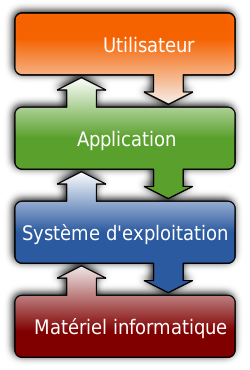
\includegraphics[height=6cm]{../illustration/OS_placement.png}
\end{figure}
\end{columns}
\end{frame}




\begin{frame}
\frametitle{Qu’est-ce qu’un système d’exploitation ?}
\begin{itemize}
\item Prend en charge le \textbf{matériel} de l'ordinateur
\begin{itemize}
\item depuis le démarrage de la machine
\end{itemize}

\item Liaison entre les \textbf{ressources matérielles} d'un ordinateur
et les \textbf{applications} de l'utilisateur
\begin{itemize}
\item traitement de texte, jeu vidéo…
\end{itemize}
\item Fournit un \textbf{environnement d'exécution uniforme} pour les autres programmes
\begin{itemize}
\item \textbf{machine virtuelle}
\item indépendante du matériel utilisé
\item interfaces standardisées (API)
\end{itemize}

\end{itemize}
\end{frame}



\begin{frame}
\frametitle{Objectifs et finalités d’un système d’exploitation}
\begin{block}{Premier rôle d'un système d'exploitation}
Fournir à l'utilisateur une \textbf{machine virtuelle} et un \textbf{environnement
d'exécution} de programmes
\end{block}
\begin{itemize}
\item Rendre le système informatique \textbf{pratique à utiliser}
\item Permettre une utilisation \textbf{efficace} du matériel
\begin{itemize}
\item couche d'abstraction matérielle
\item indépendante de la configuration matérielle
\item exploitation optimale des ressources disponibles
\end{itemize}
\item Présenter à l’utilisateur un \textbf{ordinateur idéal}
\begin{itemize}
\item Fonctions de haut niveau, faciles à programmer
\end{itemize}
\end{itemize}
\end{frame}


\begin{frame}
 \frametitle{Gestion de l'information}
 \begin{itemize}
 \item Fournir une aide à la structuration :
 \begin{itemize}
 \item de programmes
 \item de données
 \end{itemize}
 \item Gérer les catalogues de données
 \item Assurer la pérennité des données
 \begin{itemize}
  \item Contrôler l'accès aux données (sécurité)
 \end{itemize}
 \end{itemize}
 \end{frame}


\begin{frame}
 \frametitle{Gestion des communications}
 \begin{itemize}
 \item Ouverture à d'autres machines virtuelles
 \begin{itemize}
 \item locales (utilisateurs)
 \item distantes
 \end{itemize}
 \item Accès à distance :
 \begin{itemize}
\item à des procédures
\item à des services
\item à des données
\end{itemize}
 \item Transfert de données
 \begin{itemize}
  \item Mobilité d'objets ou d'environnements
\end{itemize}
\end{itemize}
\end{frame}


\begin{frame}
 \frametitle{Contrôle de l'exécution}
 \begin{itemize}
 \item Assurer l'exécution de programmes
 \begin{itemize}
 \item en séquence
 \item en parallèle
 \end{itemize}
 \item Suivre leur déroulement
 \begin{itemize}
 \item concurrence, synchronisation
 \item mesure du temps
 \item réagir aux défaillances
 \begin{itemize}
 \item points de reprise
 \item procédures dégradées
 \end{itemize}
 \end{itemize}
 \item Faciliter la composition de programmes
 \begin{itemize}
 \item chaînage, enchaînement, découpage...
 \end{itemize}
 \end{itemize}
\end{frame}


\begin{frame}
 \frametitle{Niveau d'abstraction et visibilité}
Dépend du niveau d'abstraction où se place ce travail :
 \begin{itemize}
 \item<1> Au niveau d'une \textbf{application} particulière
 \begin{itemize}
 \item IHM de l'application (Interface Homme Machine)
 \end{itemize}
 \item<2> Manipulation avec \textbf{langage de commande}
 \begin{itemize}
 \item Langage de script utilisé (Shell Unix, par exemple).
 \end{itemize}
 \item<3> Programmation système à l'aide d'un \textbf{langage évolué}
 \begin{itemize}
 \item API du système (C sur POSIX, pour Unix)
 \end{itemize}
 \item<4> Exploitation d'objets du \textbf{système à distance}
 \begin{itemize}
 \item Corba, Java, DCom, SOAP...
 \end{itemize}
 \item<5> Dans le cadre de l'utilisation du \textbf{langage machine}
 \begin{itemize}
 \item Architecture processeur, conventions de l'espace d'adressage de l'OS, interruption, mode d'exécution...
 \end{itemize} 
 \end{itemize}
\end{frame}

\begin{frame}
\frametitle{Niveau d'abstraction et niveau de langage}
\begin{tabular}{c|p{4.5cm}|p{4cm}}
Niveau 5 & Couche langage orienté application & Langage de haut niveau (C, par exemple) \\
\hline
Niveau 4 & Couche langage d'assemblage & Langage assembleur \\
\hline
Niveau 3 & Couche système d'exploitation & API du système \\
\hline
Niveau 2 & Couche architecture du jeu d'instructions (ISA) & Jeu d'instruction du processeur \\
\hline
Niveau 1 & Couche micro-architecture & Instructions de base \\
\hline
Niveau 0 & Couche circuits logiques & Action directe sur le matériel (signaux électriques)\\
\end{tabular}
\end{frame}





\begin{frame}{L'API du système}
API : \textit{Application Programming Interface}
\begin{itemize}
\item Ensemble des fonctions fournies par l'OS
\item Clairement définies, immuables
\item Programme "bien écrit" :
\begin{itemize}
\item n'utilise que les API du système
\item possibilité de fonctionner sur toutes les machines sur lesquelles le système est installé et fonctionne
\end{itemize}
\end{itemize}
\begin{block}<2>{Du point de vue du programmeur}
Système d'exploitation = ensemble de fonctions appelables, permettant de manipuler les ressources logiques et physiques du système
\end{block}
\end{frame}


\begin{frame}
\frametitle{Les systèmes d'exploitation les plus connus}
\begin{itemize}
\item Grand public :
\begin{itemize}
\item Windows / Phone / RT, MacOS X / iOS, Linux / Android
\end{itemize}
\item Serveur et mini (moyens systèmes) :
\begin{itemize}
\item Dérivés d'UNIX :
\begin{itemize}
\item GNU/Linux ou Hurd
\item BSD : NetBSD, OpenBSD, FreeBSD, Darwin
\item UNIX propriétaires : AIX, Irix, HP-UX, Solaris, Sinix, Tru64
\end{itemize}
\item OS/400 (AS/400 - iSeries), VMS et OpenVMS
\end{itemize}
\item Grands systèmes (mainframes) :
\begin{itemize}
\item IBM: MVS, VM, DOS/VSE, TPF - Bull: GCOS - Siemens: BS2000 - MULTICS
\end{itemize}
\item Systèmes spéciaux :
\begin{itemize}
\item Symbian OS, Pixo, LynxOS, Minix, QNX...
\end{itemize}
\end{itemize}
\end{frame}


\begin{frame}
\frametitle{Composition d'un système d'exploitation}
\begin{itemize}
\item Un noyau
\item Un ensemble de bibliothèques dynamiques, exploitables via l'API du système
\item Un ensemble d'outils système
\item Des programmes applicatifs de base
\end{itemize}
\end{frame}


\begin{frame}
\frametitle{Structure fonctionnelle des systèmes d'exploitation}
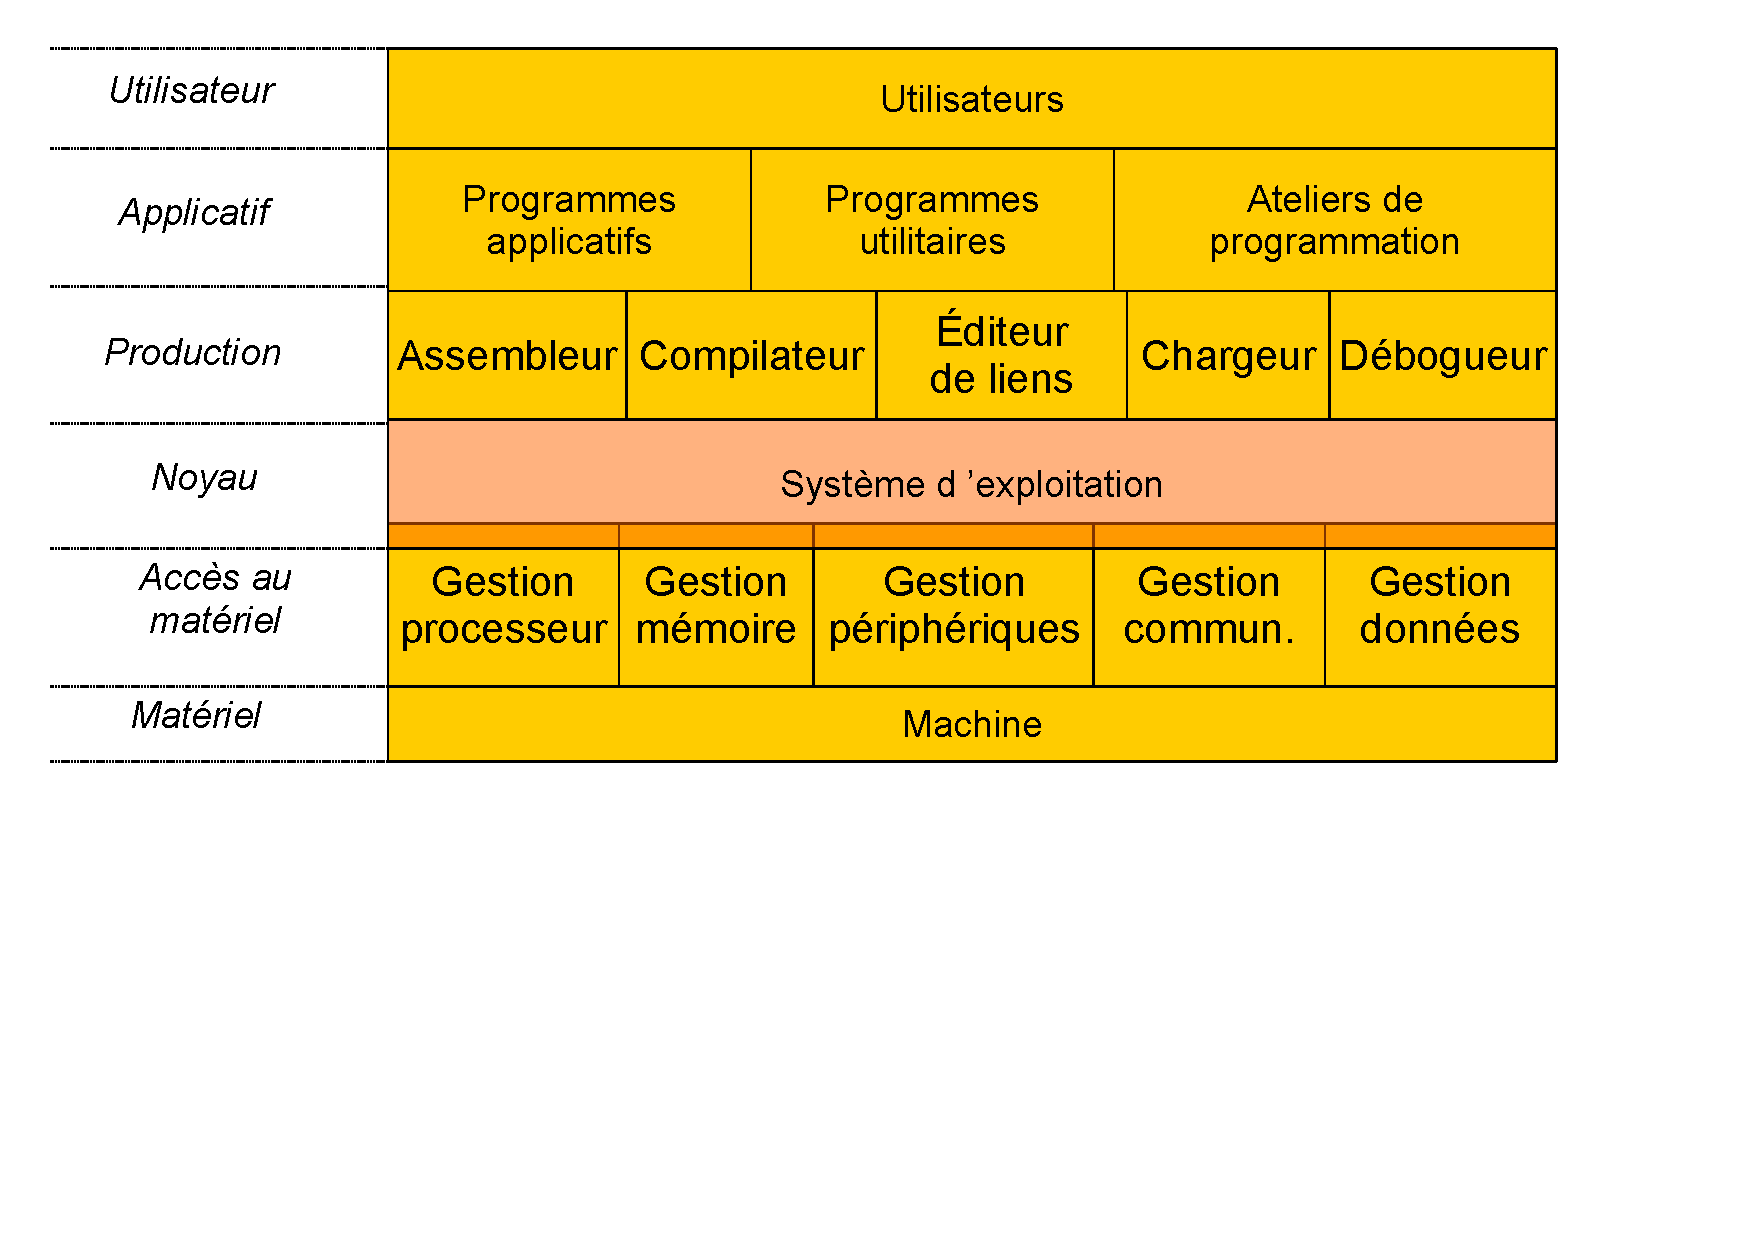
\includegraphics[width=11cm]{../illustration/structure_fonctionnelle.pdf}
\end{frame}

\begin{frame}
\frametitle{Structure technique du noyau}
\begin{itemize}
\item Monolithique
\item A couches
\item Client-serveur
\item Micro-noyau
\item Machines virtuelles
\end{itemize}
\end{frame}


\subsection{Structure monolithique}

\begin{frame}
\frametitle{Structure monolithique}
Toutes les fonctionnalités regroupées dans un seul gros exécutable
\begin{itemize}
\item Pas de structure bien définie
\begin{itemize}
\item Souvent simple (à l’origine)

Exemple : MS-DOS 1.0 $\rightarrow$ 8ko, 2.0 $\rightarrow$ 24 ko, 3.0 $\rightarrow$ 36 ko... Windows ME ?
\end{itemize}
\item Bonnes performances
\item Complexe :
\begin{itemize}
\item à maintenir, à faire évoluer, à fiabiliser (effets de bord)
\end{itemize}
\end{itemize}
\begin{exampleblock}<2>{Exemples d'OS à structure monolithique}
\textbf{MS-DOS}, mais aussi \textbf{Linux} (structuration rigoureuse des sources et noyau modulable)
\end{exampleblock}
\end{frame}


\begin{frame}
\frametitle{Structure monolithique}
\begin{columns}
\column{.5\textwidth}
\begin{block}{Avantages}
\begin{itemize}
\item Structure simple
\item Performances optimales
\item Partage de données facilité
\end{itemize}
\end{block}
\column{.5\textwidth}
\begin{block}{Inconvénients}
\begin{itemize}
\item Difficile à maintenir
\item Effets de bords
\item Difficile à fiabiliser
\end{itemize}
\end{block}
\end{columns}
\end{frame}


\subsection{Structure à couches}

\begin{frame}
\frametitle{Structure à couches}
Décomposition en couches successives :
\begin{itemize}
\item Couche la plus basse (0) : 
\begin{itemize}
\item matériel
\end{itemize}

\item Couche la plus haute :
\begin{itemize}
\item utilisable par les applications
\end{itemize}

\item Contraintes :
\begin{itemize}
\item Couche (n) peut uniquement faire appel aux fonctionnalités de la couche (n-1)
\item Cloisonnement du fonctionnement interne des couches
\end{itemize}
\end{itemize}
\end{frame}


\begin{frame}
\frametitle{Struture à couche}
\begin{center}
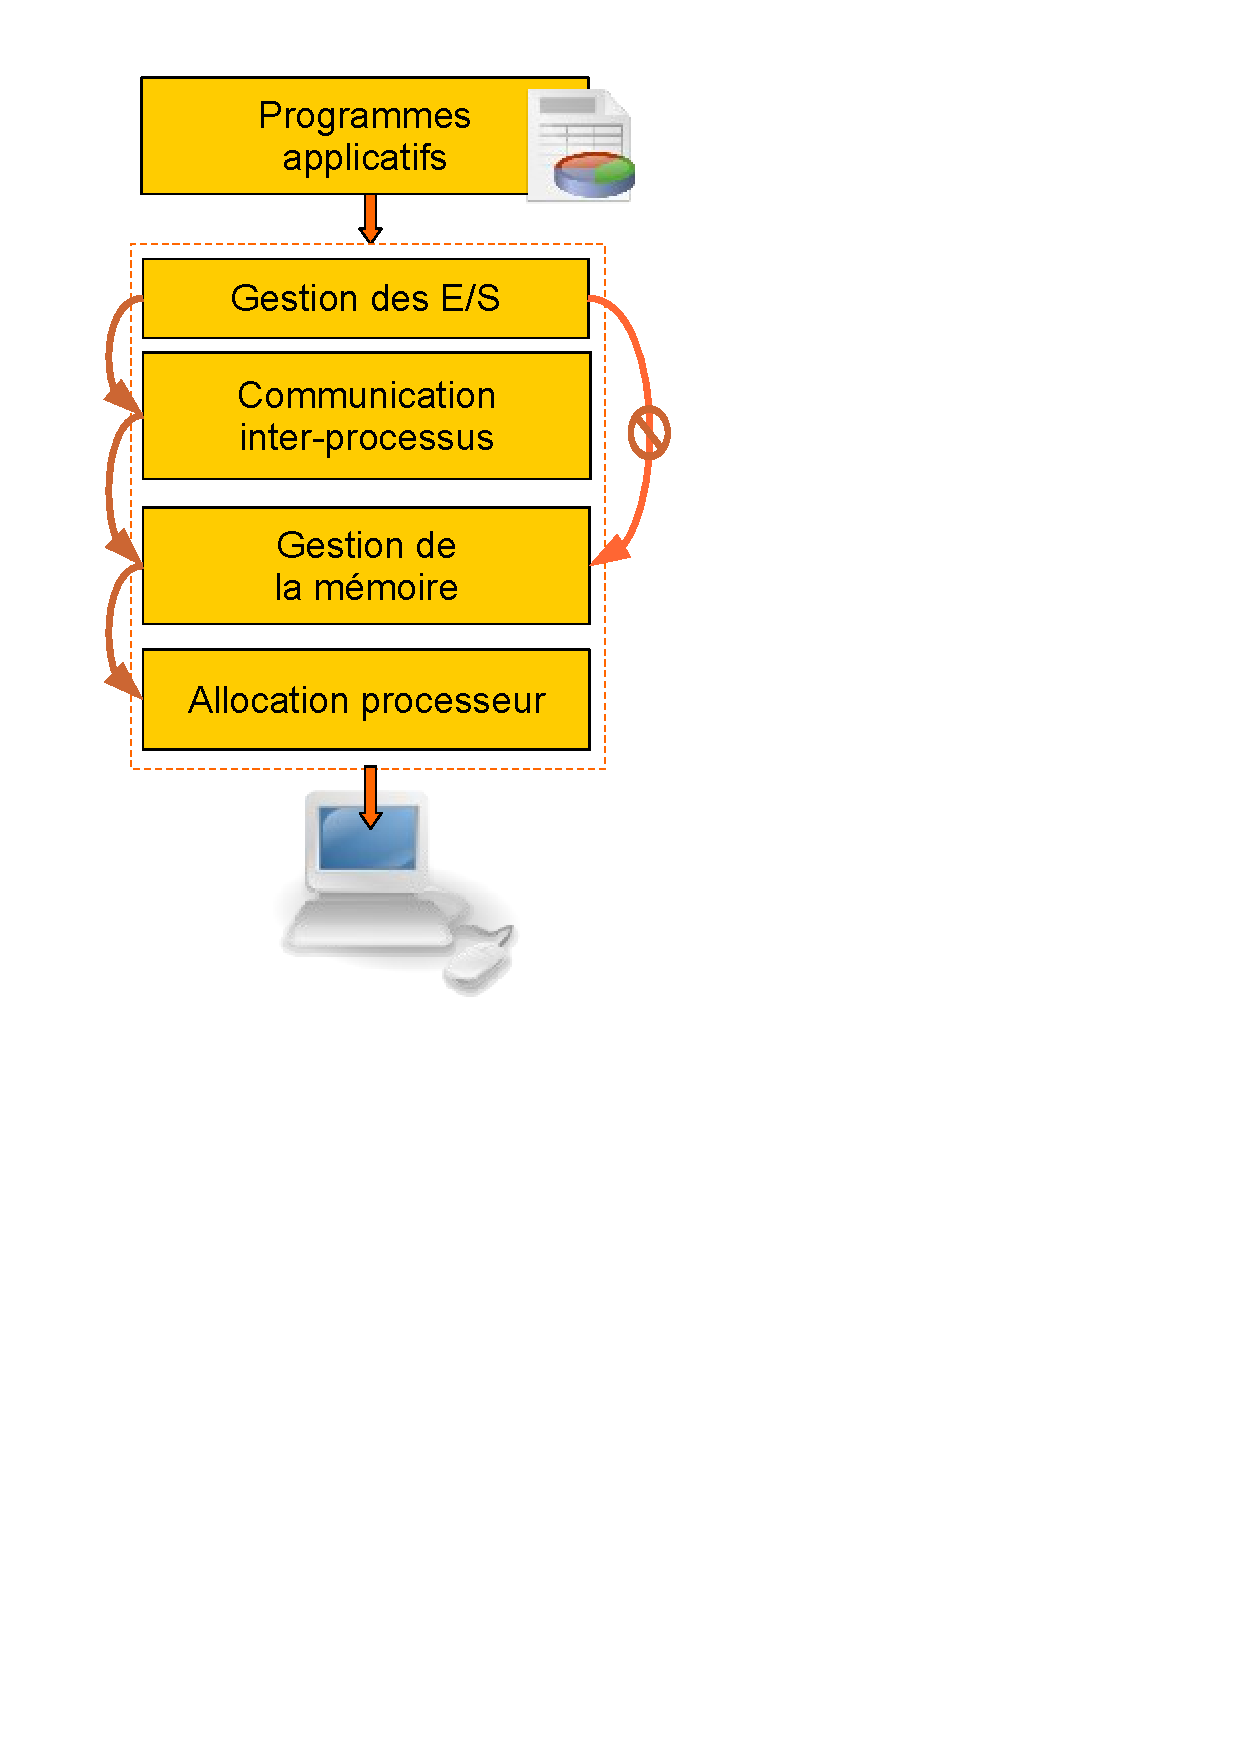
\includegraphics[height=6.5cm]{../illustration/modele_couche.pdf}
\end{center}
\end{frame}


\begin{frame}
\frametitle{Structure à couches}
\begin{columns}
\column{.5\textwidth}
\begin{block}{Avantages}
\begin{itemize}
\item Élève progressivement le niveau d’abstraction
\item Facilite la mise au point
\item Facilite le portage
\item Augmente la sécurité
\end{itemize}
\end{block}
\column{.5\textwidth}
\begin{block}{Inconvénients}
\begin{itemize}
\item Nécessite une conception fine de la structure au préalable
\item Perte d’efficacité (communications)
\item Rigidité
\end{itemize}
\end{block}
\end{columns}
\end{frame}

\begin{frame}
\frametitle{Exemple : OS/2 d'IBM}
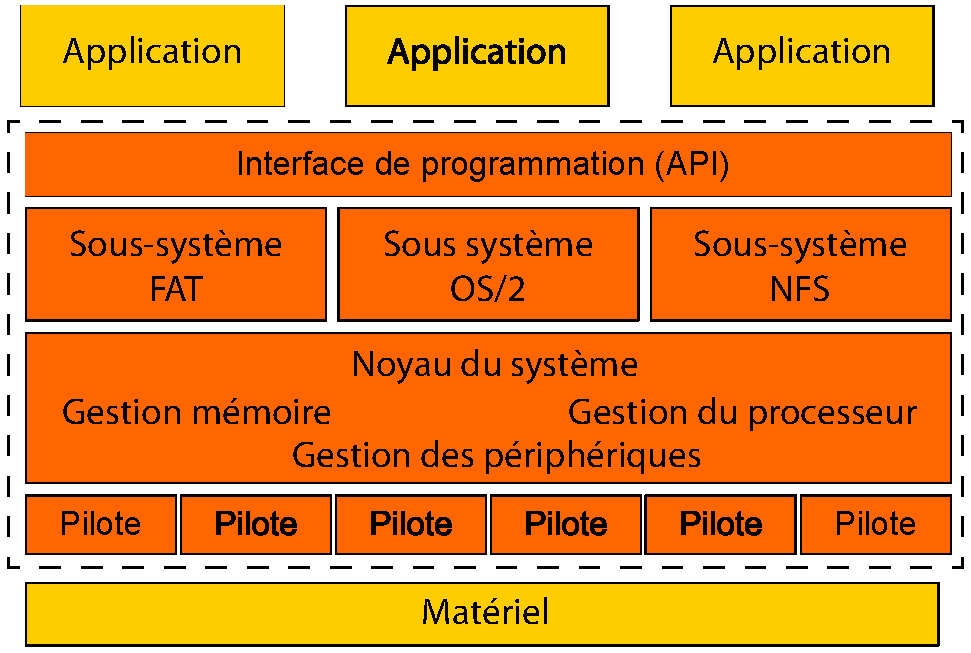
\includegraphics[height=6cm]{../illustration/exemple_os2.pdf}
\end{frame}


\subsection{Structure client-serveur}

\begin{frame}
\frametitle{Structure client-serveur}
\begin{itemize}
\item Enlever les composants non essentiels du noyau
\item Les implémenter comme des programmes
\item Communication par passage de messages
\end{itemize}
\begin{exampleblock}<2>{Exemple d'OS à structure client-serveur}
Windows NT
\end{exampleblock}
\end{frame}


\begin{frame}
\frametitle{Exemple : Windows NT}
\begin{center}
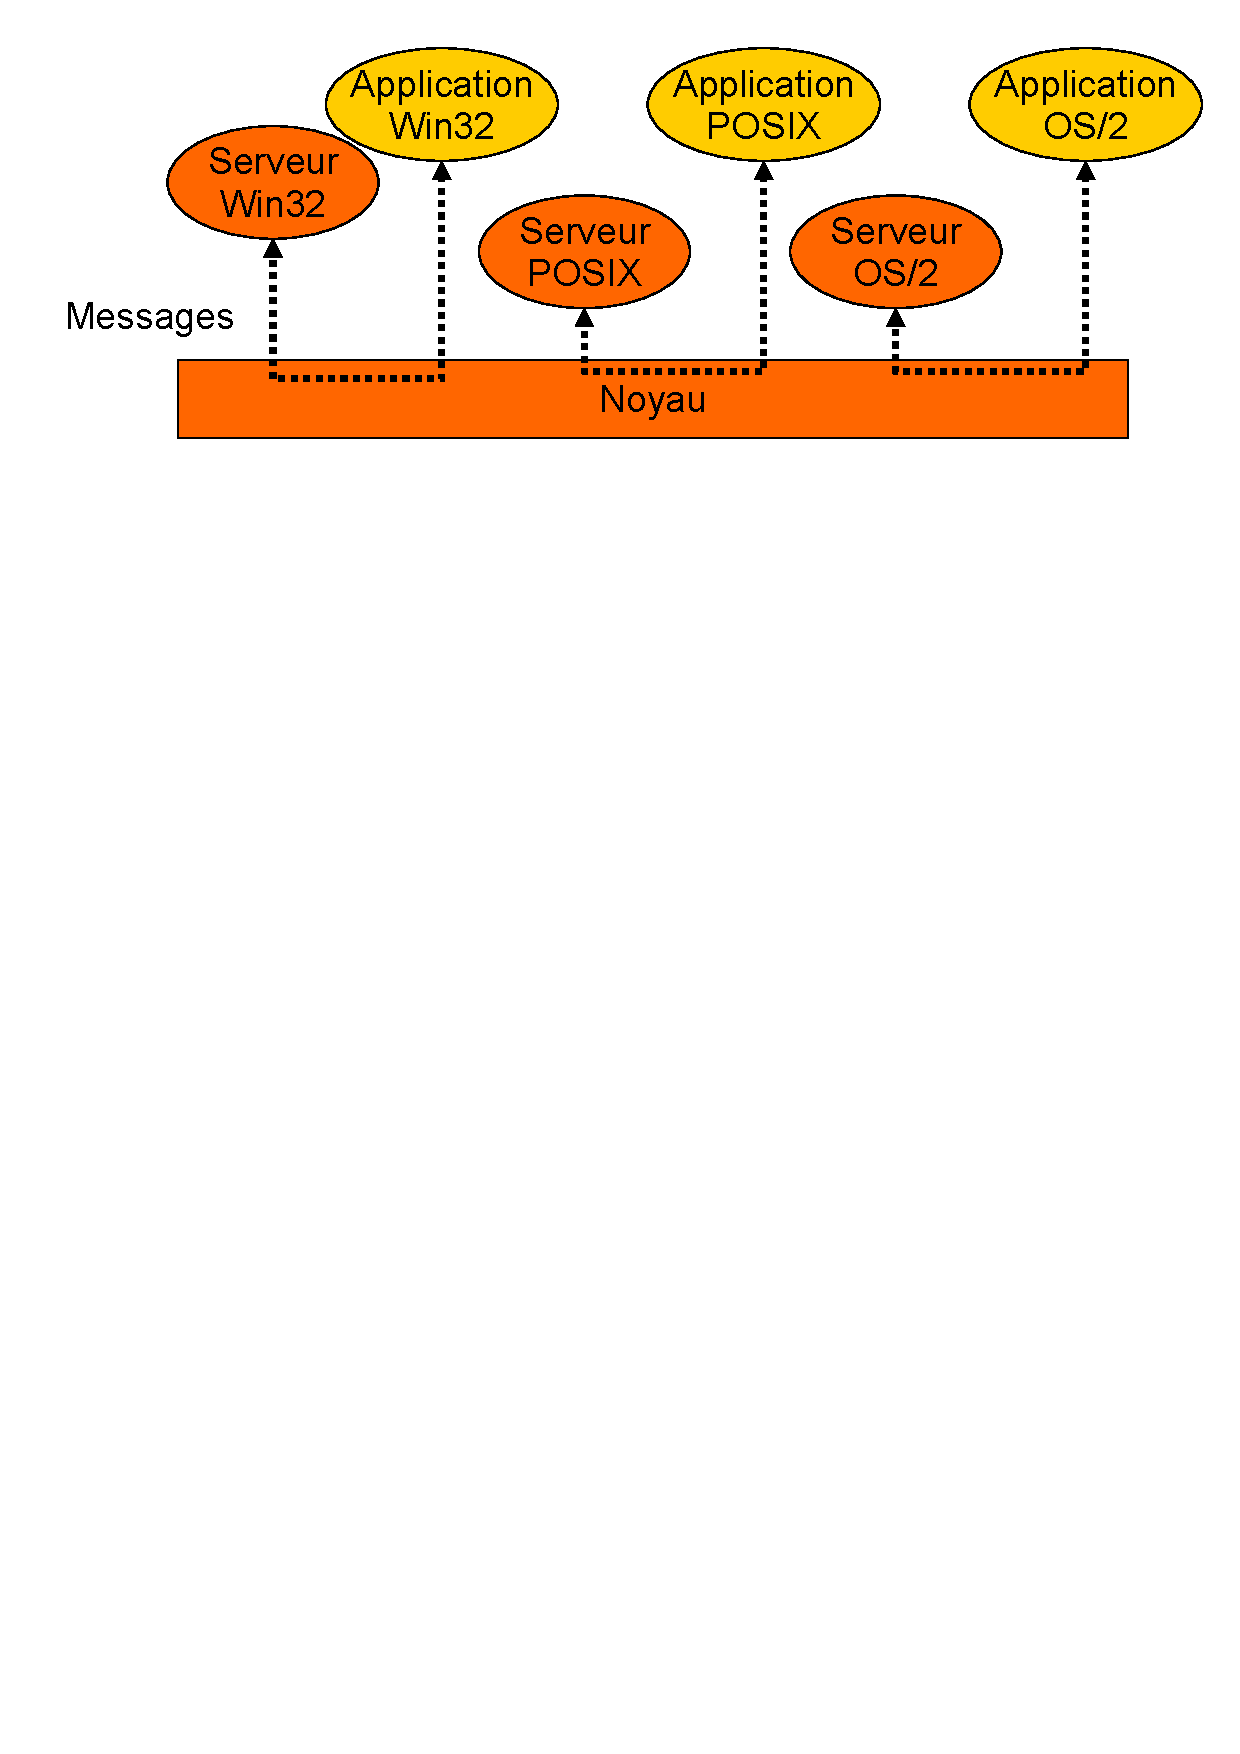
\includegraphics[width=11.5cm]{../illustration/exemple_winnt.pdf}
\end{center}
\end{frame}


\begin{frame}
\frametitle{Structure client-serveur}
\begin{columns}
\column{.5\textwidth}
\begin{block}{Avantages}
\begin{itemize}
\item Évolutivité, facilité de maintenance
\item Adaptabilité, portabilité
\item Stabilité, sécurité
\end{itemize}
\end{block}
\column{.5\textwidth}
\begin{block}{Inconvénients}
\begin{itemize}
\item Perte de performance (communications)
\item Goulot d’étranglement sur le noyau
\item Communication inter module
\end{itemize}
\end{block}
\end{columns}

\begin{center}
\textit{Microsoft a remis en cause cette organisation rigoureuse en ré-intégrant beaucoup de fonctions dans le noyau à partir de Windows NT4}
\end{center}
\end{frame}


\subsection{Structure à micro-noyau}

\begin{frame}
\frametitle{Structure à micro-noyau}
\begin{itemize}
\item Noyau réduit à sa plus simple expression
\begin{itemize}
\item Gestion mémoire
\item Gestion des travaux
\item Fonctions de communication
\end{itemize}
\item Les autres fonctions sont déportées hors du noyau
\end{itemize}
\begin{exampleblock}<2>{Exemples d'OS à micro-noyau}
\begin{itemize}
\item BeOs, Minix, Hurd - Mach, QNX

\item MacOs X : Darwin basé sur l'implémentation BSD (FreeBSD) du micro-noyau Mach
\begin{itemize}
\item Serveur FreeBSD sur micro-noyau Mach
\item Fusion des deux éléments
\end{itemize}
\end{itemize}


\end{exampleblock}
\end{frame}


\begin{frame}
\frametitle{Structure à micro-noyau}
\begin{columns}
\column{.5\textwidth}
\begin{block}{Avantages}
\begin{itemize}
\item Modularité
\begin{itemize}
\item Facilement parallélisable
\end{itemize}
\item L'évolutivité
\begin{itemize}
\item Stabilité
\item Facilité de maintenance
\end{itemize}
\item Adaptabilité
\begin{itemize}
\item Portabilité
\item S'adapte à un large panel de besoins
\end{itemize}
\end{itemize}
\end{block}
\column{.5\textwidth}
\begin{block}{Inconvénients}
\begin{itemize}
\item Complexité
\item Communications coûteuses
\item Perte d'efficacité
\begin{itemize}
\item goulot d'étranglement sur le micro-noyau
\end{itemize}
\end{itemize}
\end{block}
\end{columns}
\end{frame}



\section{Processus et contexte d'exécution}
\subsection{La notion de processus}

\begin{frame}
\frametitle{La notion de processus}
\begin{itemize}
\item Premiers systèmes :
\begin{itemize}
\item Exécution d’un seul programme à la fois
\item Dispose de toutes les ressources
\item Pas de concurence
\end{itemize}
\item Systèmes actuels :
\begin{itemize}
\item Plusieurs programmes s’exécutent simultanément
\item Entrent en concurrence pour l’utilisation des ressources
\item Notion de processus
\end{itemize}
\item Le système prend en charge des \emph{processus}
\end{itemize}
\end{frame}

\begin{frame}
\frametitle{Définition d’un processus}
\begin{itemize}
\item Programme en exécution
\begin{itemize}
\item activité séquentielle
\item en concurrence avec d'autres
\item change d’état au cours de son exécution
\end{itemize}
\item Nécessite des ressources
\begin{itemize}
\item au moins CPU + mémoire
\end{itemize}
\item Contexte d'exécution propre
\begin{itemize}
\item mémoire dédiée
\item exécution indépendante
\item représenté par un bloc de contrôle (PCB)
\end{itemize}
\end{itemize}
\end{frame}


\begin{frame}
\frametitle{Qu'est-ce qu'un processus ?}
\begin{itemize}
\item Concept de base de la \textbf{concurrence}
\item Entité d'affectation du processeur
\begin{itemize}
\item En dehors des traitements d'interruptions et des périodes de transition, le processeur est alloué à un processus
\item Les processus peuvent prendre deux états : 
\begin{itemize}
\item ils sont \textbf{actifs} (en exécution ou prêt à l'être)
\item ou \textbf{bloqués} (en attente d'un événement)
\end{itemize}

\end{itemize}
\item Activité autonome et, à priori, indépendante
\begin{itemize}
\item \textbf{interactions} possibles entre processus
\item \textbf{concurrence} pour l'accès aux ressources
\end{itemize}
\end{itemize}
\end{frame}

\subsection{Contexte d'exécution indépendant}

\begin{frame}
\frametitle{Bloc de contrôle d’un processus (PCB)}
\begin{columns}
\column{0.4\textwidth}
\begin{itemize}
\item Stockage des informations pouvant varier d’un processus à l’autre
\item Contient le PSW
\begin{itemize}
\item Program Status Word
\end{itemize}
\end{itemize}
\column{0.6\textwidth}
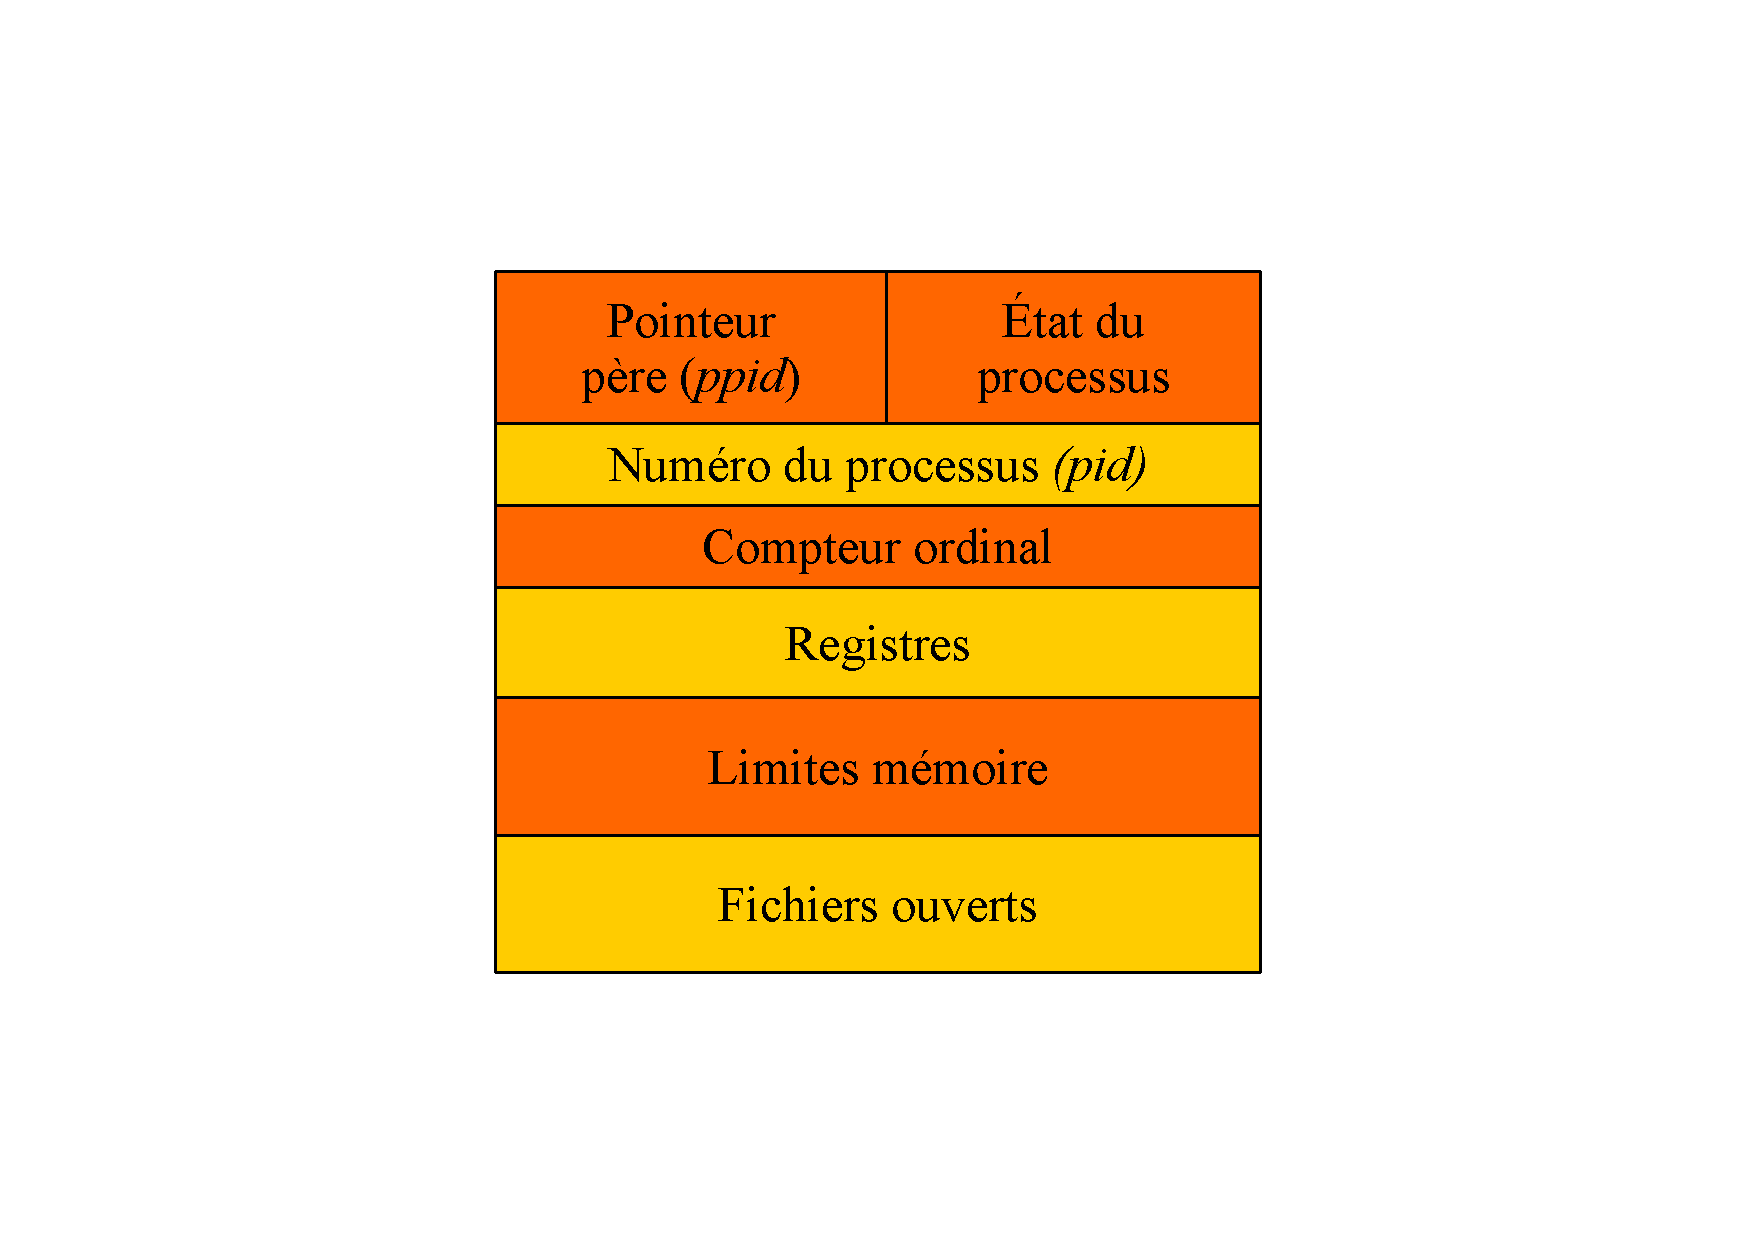
\includegraphics[width=5cm]{../illustration/PCB.pdf}
\end{columns}
\end{frame}

\begin{frame}
\frametitle{Commutation de contexte}
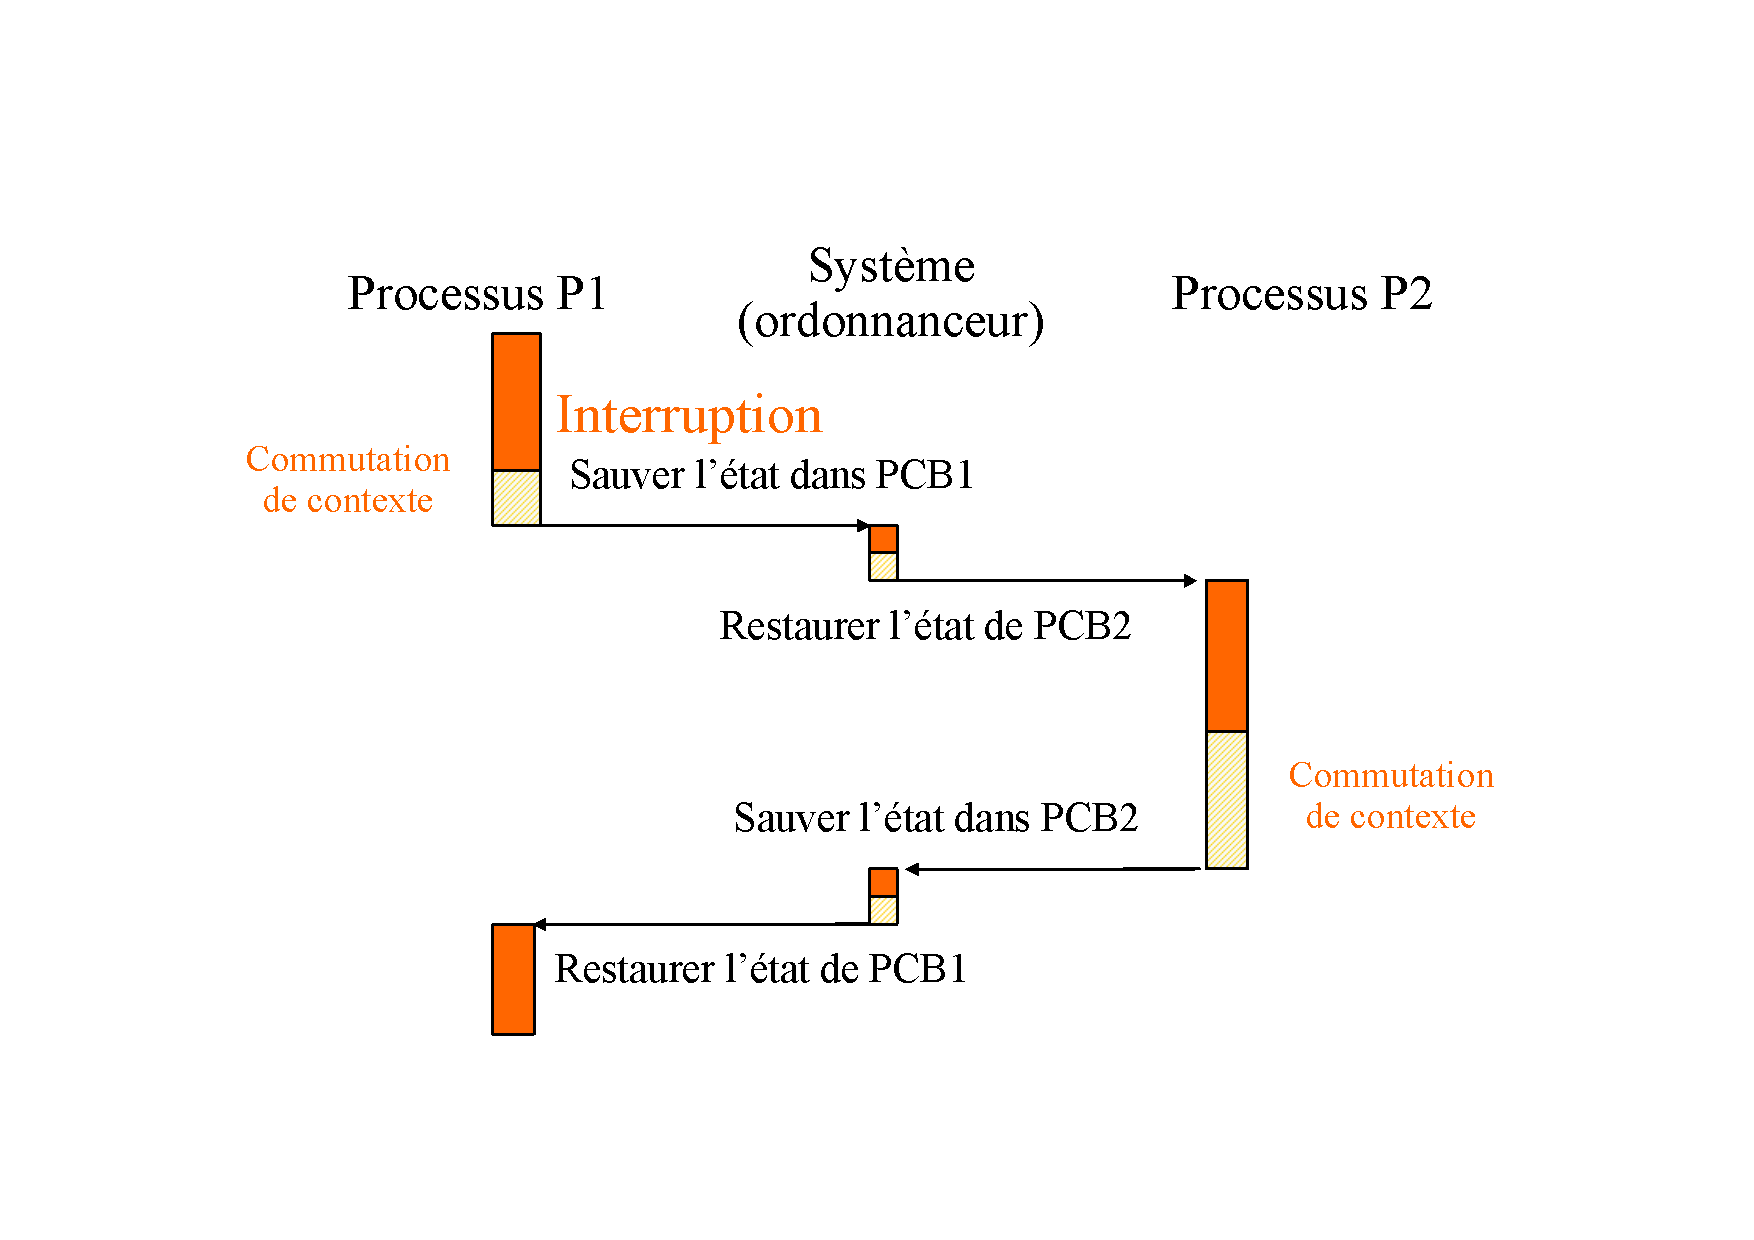
\includegraphics[height=5cm]{../illustration/commutation_contexte.pdf}
\end{frame}

\subsection{Cycle de vie}

\begin{frame}
\frametitle{Hiérarchie des processus}
\begin{itemize}
\item Premier processus créé au démarrage du système
\begin{itemize}
\item Ancêtre de tous les autres processus
\end{itemize}
\item Chaque processus peut en créer d’autres
\item Chaque processus est créé par un autre processus (sauf le premier)
\begin{itemize}
\item Processus père
\item Hiérarchie des processus
\item Le fils hérite du contexte de son père
\end{itemize}
\end{itemize}
\end{frame}


\begin{frame}
\frametitle{Hiérarchie des processus}
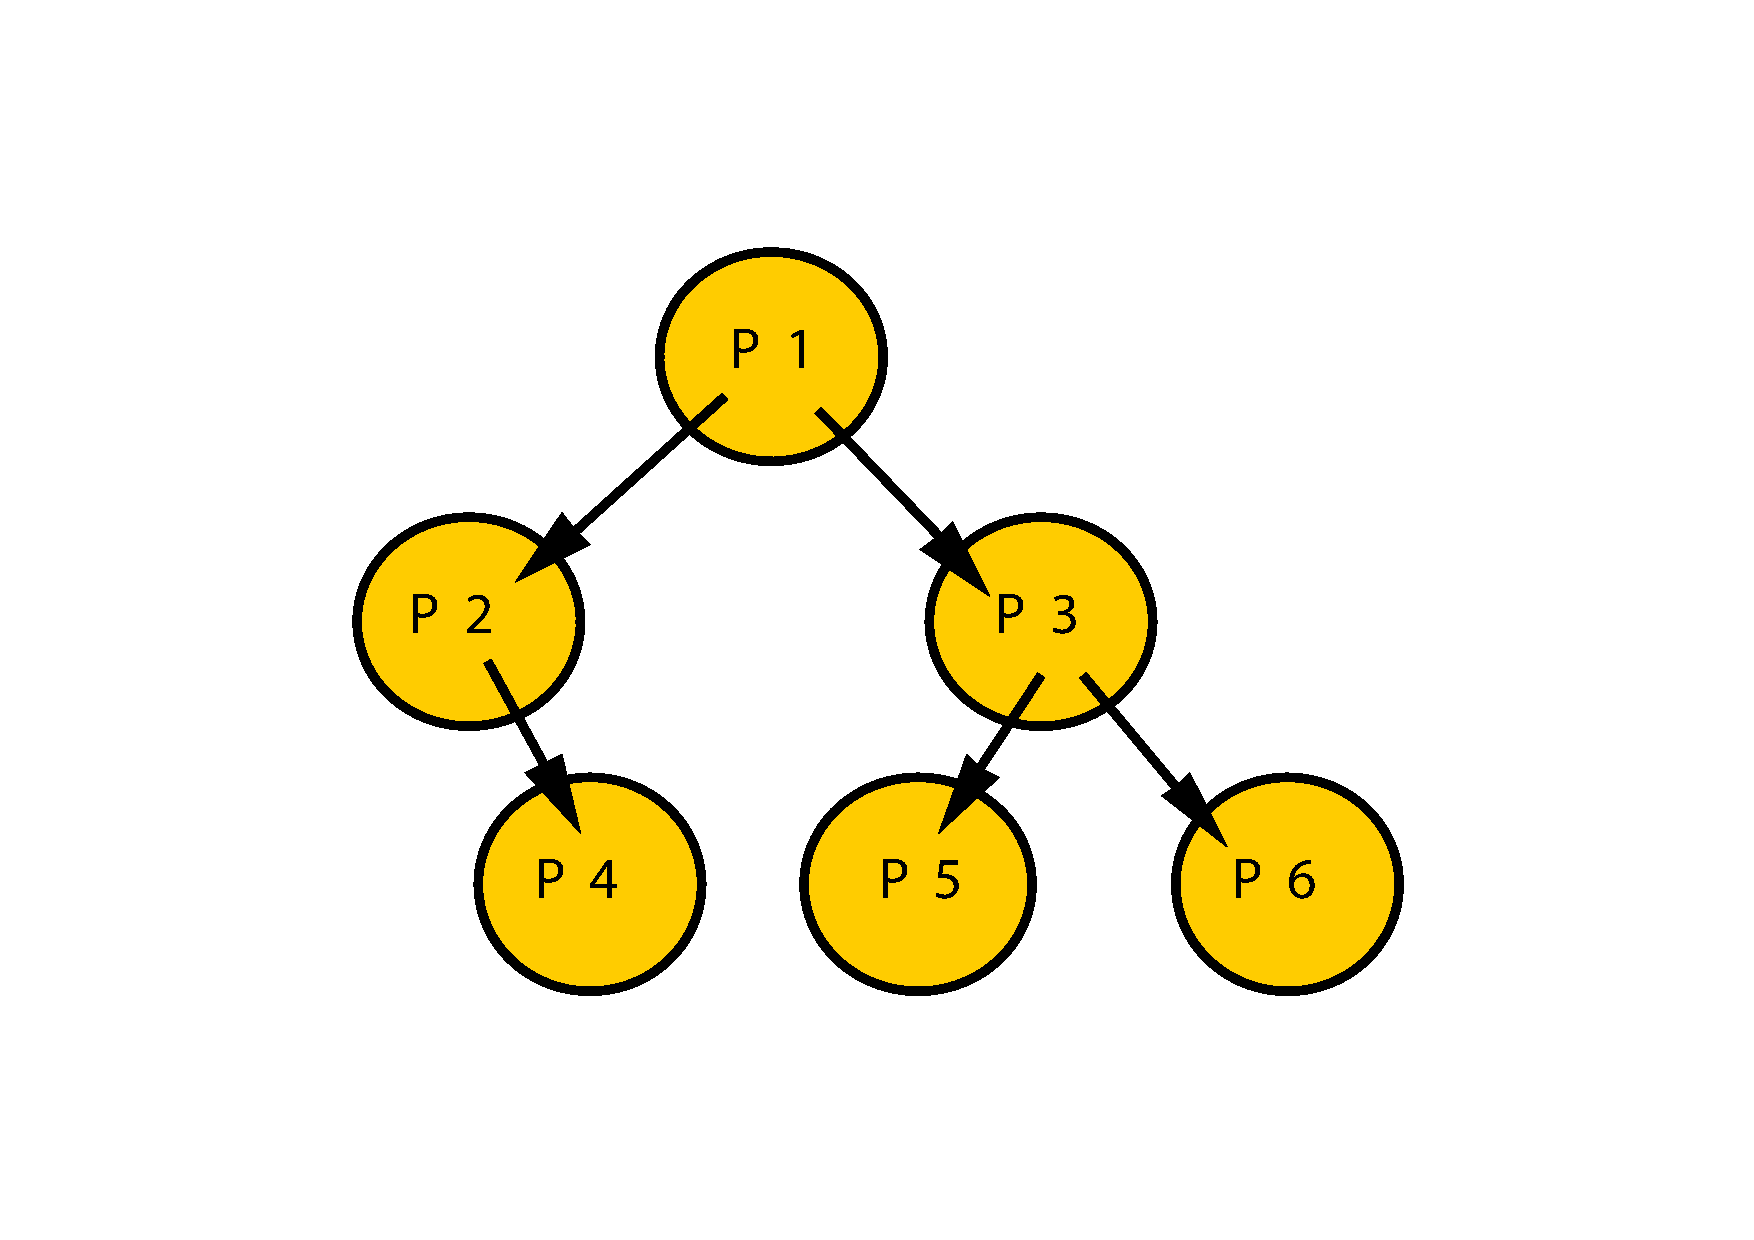
\includegraphics[height=5cm]{../illustration/process_hierarchie.pdf}
\end{frame}


\begin{frame}
\frametitle{Cycle de vie d'un processus}
\begin{itemize}
\item Trois états :
\begin{itemize}
\item Processus actif, en exécution (\textbf{Élu})
\begin{itemize}
\item Dispose de la CPU
\end{itemize}
\item Suspendu en attente d’exécution (\textbf{Prêt})
\begin{itemize}
\item Attend la CPU
\end{itemize}
\item En attente d’un événement (\textbf{Bloqué})
\begin{itemize}
\item Libération de ressource autre que la CPU
\item Événement interne ou externe
\end{itemize}
\end{itemize}
\end{itemize}
\end{frame}

\begin{frame}
\frametitle{Cycle de vie d'un processus}
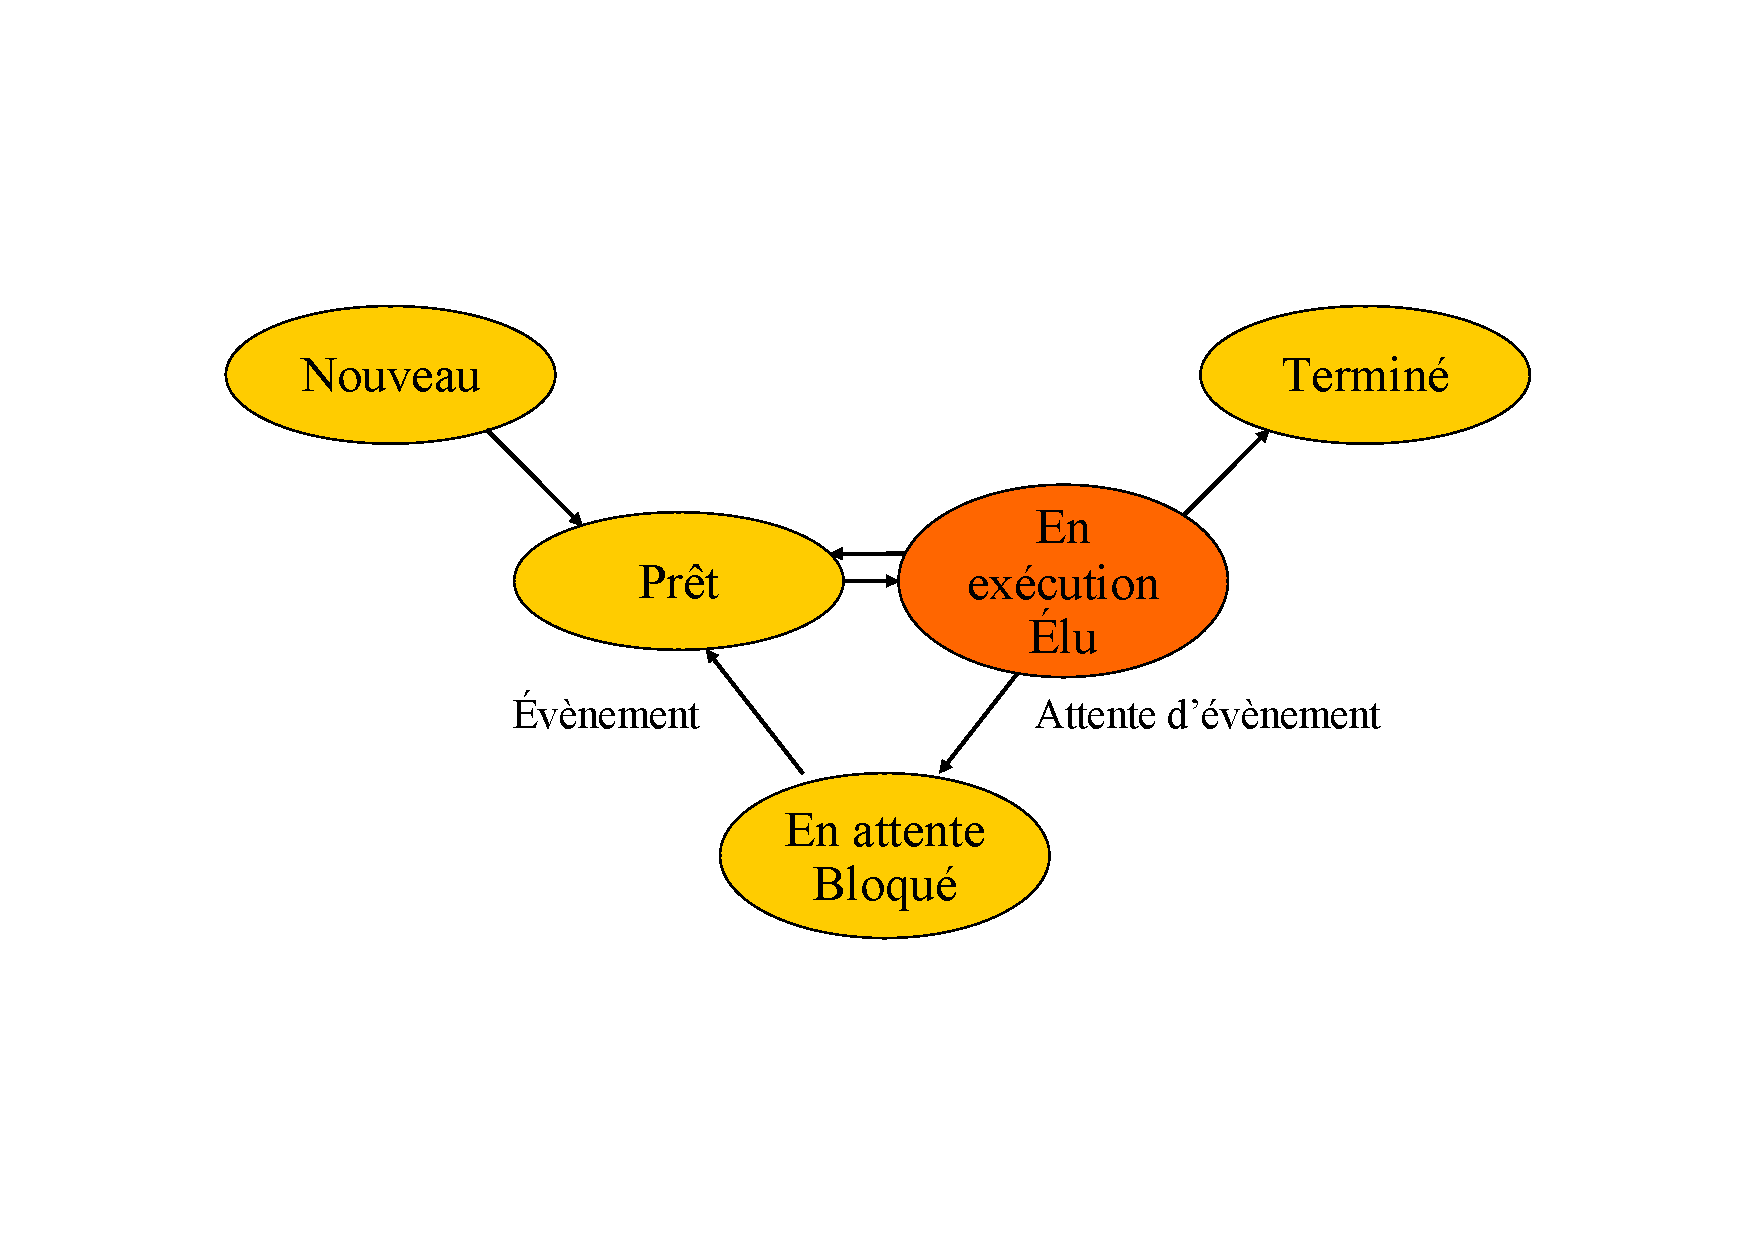
\includegraphics[height=5cm]{../illustration/process_cycle_vie.pdf}
\end{frame}


\begin{frame}
\frametitle{Création de processus}
\begin{itemize}
\item Appel système depuis un processus
\begin{itemize}
\item Devient le père du nouveau processus
\item Ajout d'une d’une feuille à l’arbre des processus
\end{itemize}
\item Le nouveau processus est un clone de son père
\begin{itemize}
\item Exécute le même programme
\item Dispose d'une copie de toutes les données
\item Héritage des ressources du père
\item Seul le numéro de processus est différent
\end{itemize}
\item Entre en concurrence avec le père
\end{itemize}
\end{frame}


\begin{frame}
\frametitle{Terminaison de processus}
\begin{itemize}
\item Appel système
\item Retour d’information vers le père
\item Libération des ressources
\end{itemize}
\begin{block}{Cas de terminaison}
\begin{itemize}
\item Exécution de la dernière instruction
\item Appel système 
\begin{itemize}
\item depuis le processus lui-même
\item depuis un autre processus (souvent le père)
\end{itemize}
\item Terminaison du père (terminaison en cascade)
\end{itemize}
\end{block}
\end{frame}


\begin{frame}
\frametitle{La primitive \texttt{fork()}}
\begin{itemize}
\item <1> Création d’un clone du processus père
\begin{itemize}
\item Même contexte :
\begin{itemize}
\item Même vue du code
\item Mêmes fichiers ouverts
\item Même environnement
\end{itemize}
\item Seules différences : \texttt{pid} et \texttt{ppid}.
\end{itemize}
\item <2> Optimisation :
\begin{itemize}
\item Duplication mémoire le plus tard possible
\begin{itemize}
\item \texttt{Copy on write}
\item Exploite les mêmes zones mémoire tant que possible
\item Duplication des seules zones modifiées
\end{itemize}
\end{itemize}
\end{itemize}
\end{frame}

\begin{frame}
\frametitle{La primitive \texttt{fork()}}
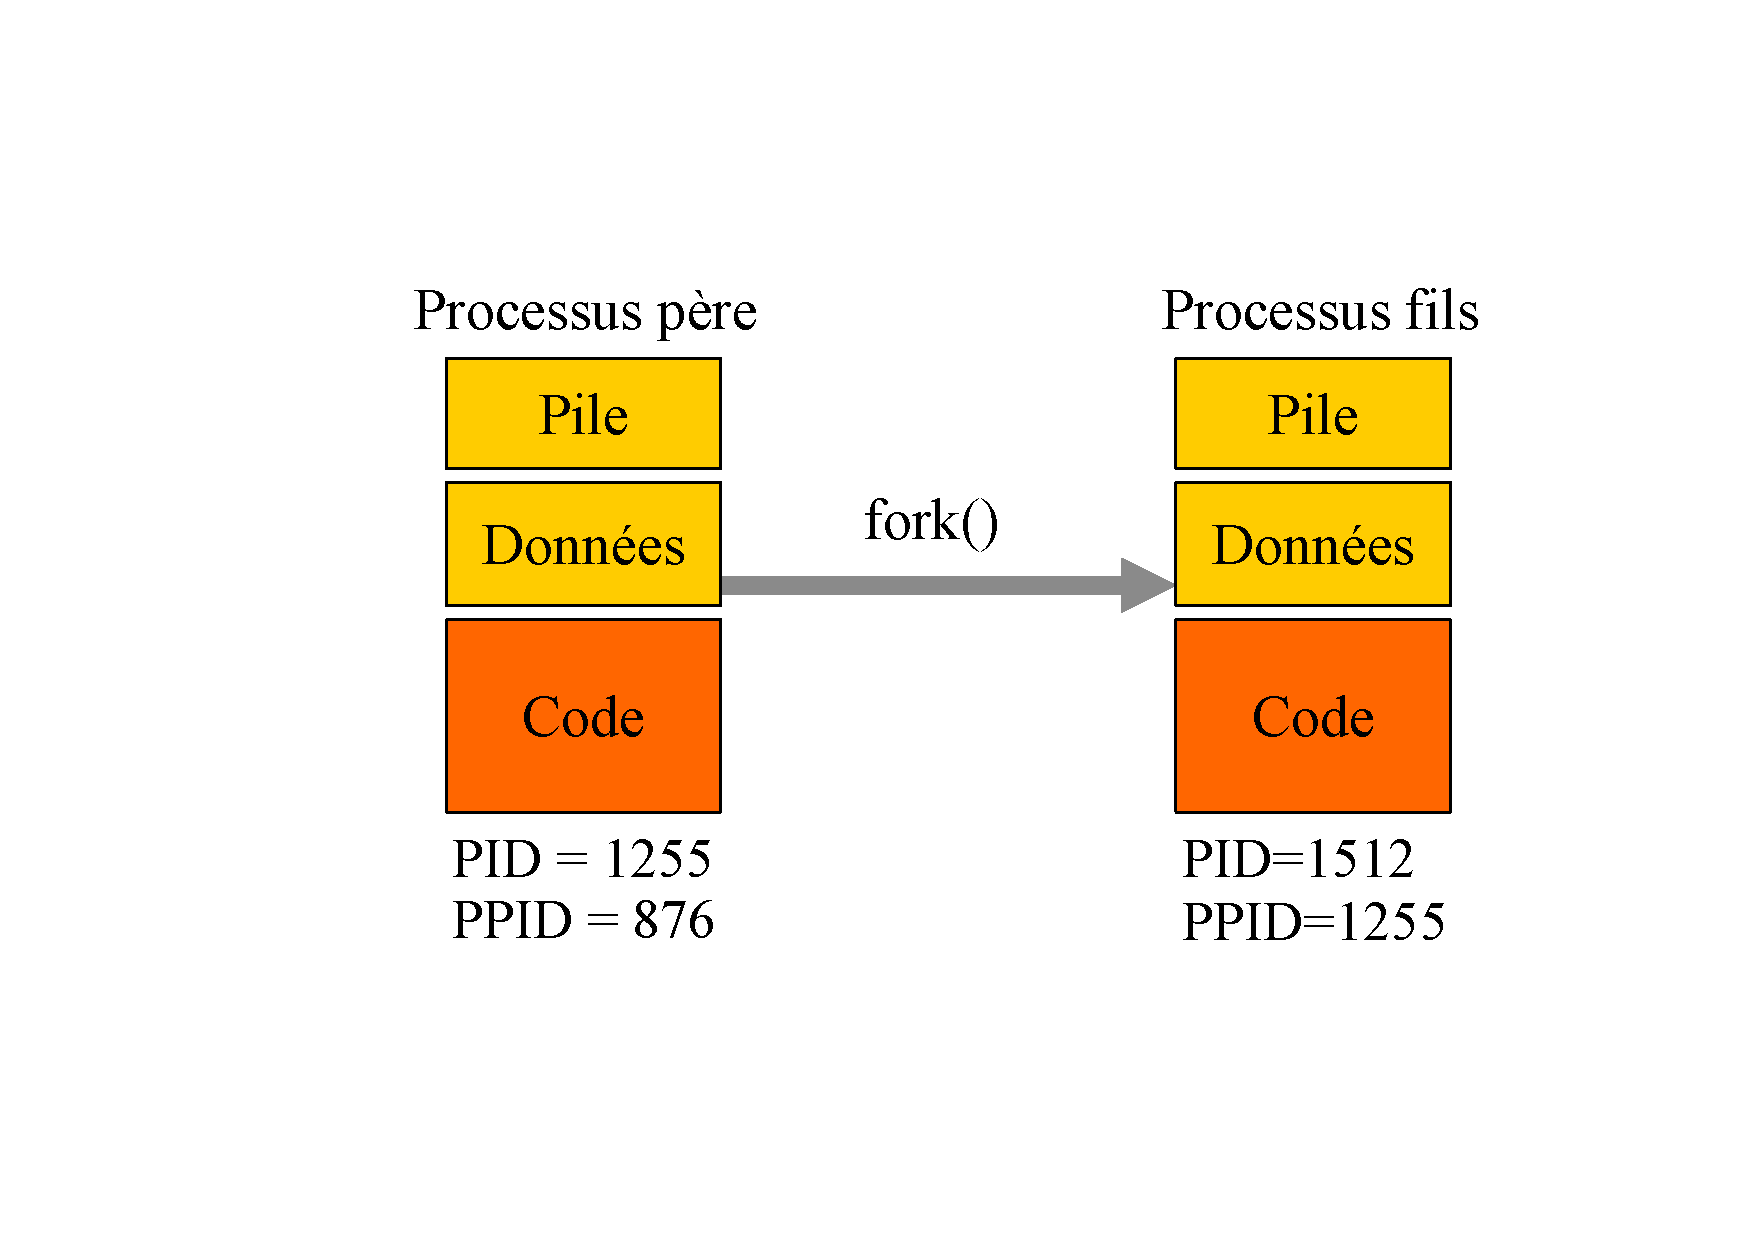
\includegraphics[height=5cm]{../illustration/fork.pdf}
\end{frame}


\begin{frame}
\frametitle{La primitive \texttt{fork()}}
\begin{columns}
\column{.6\textwidth}
\begin{small}
\verbatiminput{include/fork.c}
\end{small}
\column{.4\textwidth}
\begin{block}<only@2->{Execution}
\begin{tiny}
Exemple d'utilisation de la fonction \texttt{fork()}

retour=15330 $\rightarrow$ a=0

retour=    0 $\rightarrow$ a=0

retour=    0 $\rightarrow$ a=1

retour=15330 $\rightarrow$ a=1

retour=15330 $\rightarrow$ a=2

retour=    0 $\rightarrow$ a=2

retour=15330 $\rightarrow$ a=3

retour=    0 $\rightarrow$ a=3

retour=15330 $\rightarrow$ a=4

retour=    0 $\rightarrow$ a=4

En fin de compte, retour=0, a=5

En fin de compte, retour=15330, a=5
\end{tiny}
\end{block}
\end{columns}
\end{frame}


\begin{frame}
\frametitle{La primitive \texttt{exec()}}
\begin{itemize}
\item Charger un nouveau code exécutable
\begin{itemize}
\item Remplace le programme du père
\item Les données sont conservées
\item Permet le passage de données au fils
\end{itemize}
\item Six primitives d’appel, en fonction :
\begin{itemize}
\item Passage d’arguments (tableau, liste),
\item Spécification du chemin d’accès,
\item Modification de l’environnement
\end{itemize}
\end{itemize}
\end{frame}


\begin{frame}[fragile]
\frametitle{La primitive \texttt{exec()}}
\begin{small}
\verbatiminput{include/exec.c}
\end{small}
\end{frame}


\begin{frame}
\frametitle{Les primitives \texttt{fork()} et \texttt{exec()}}
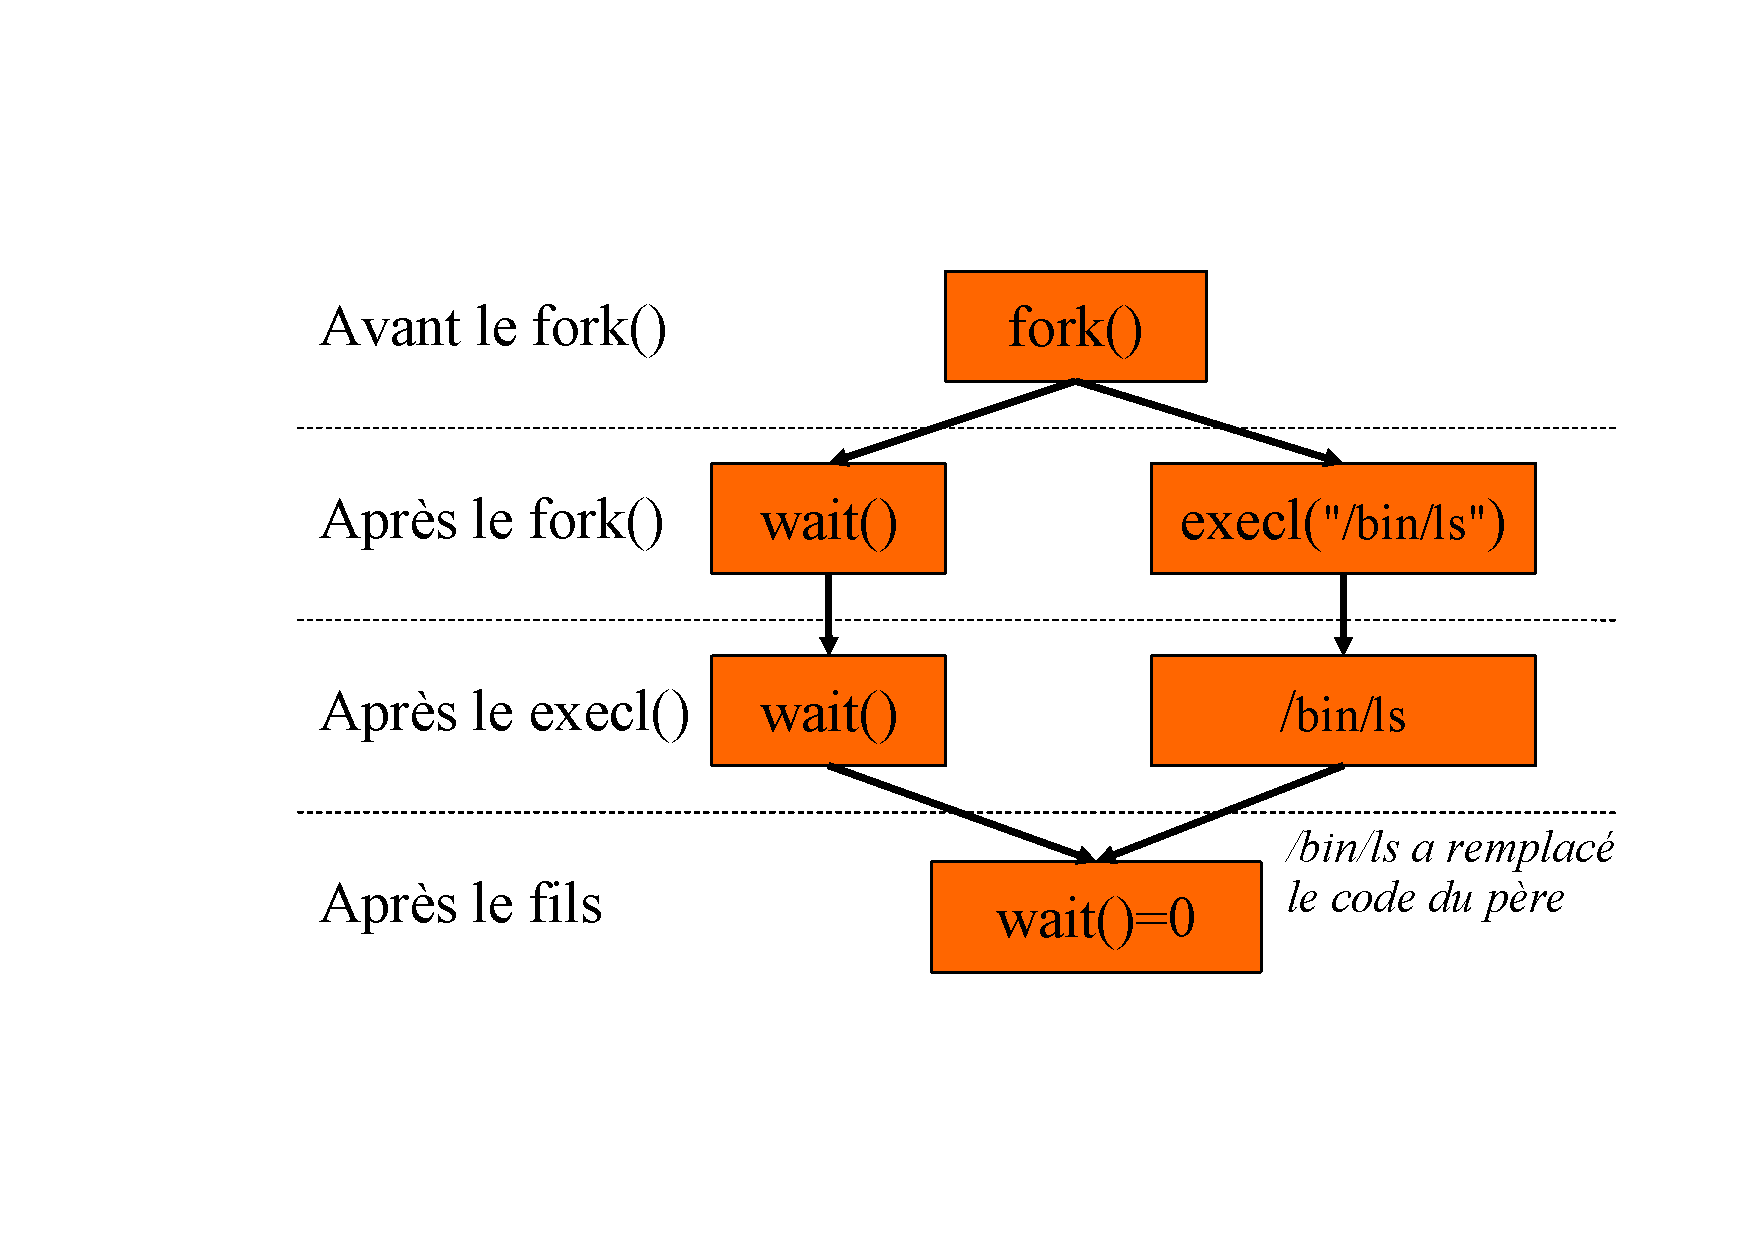
\includegraphics[height=5cm]{../illustration/fork_exemple.pdf}
\end{frame}


\begin{frame}
\frametitle{Lancement commande par un interpréteur}
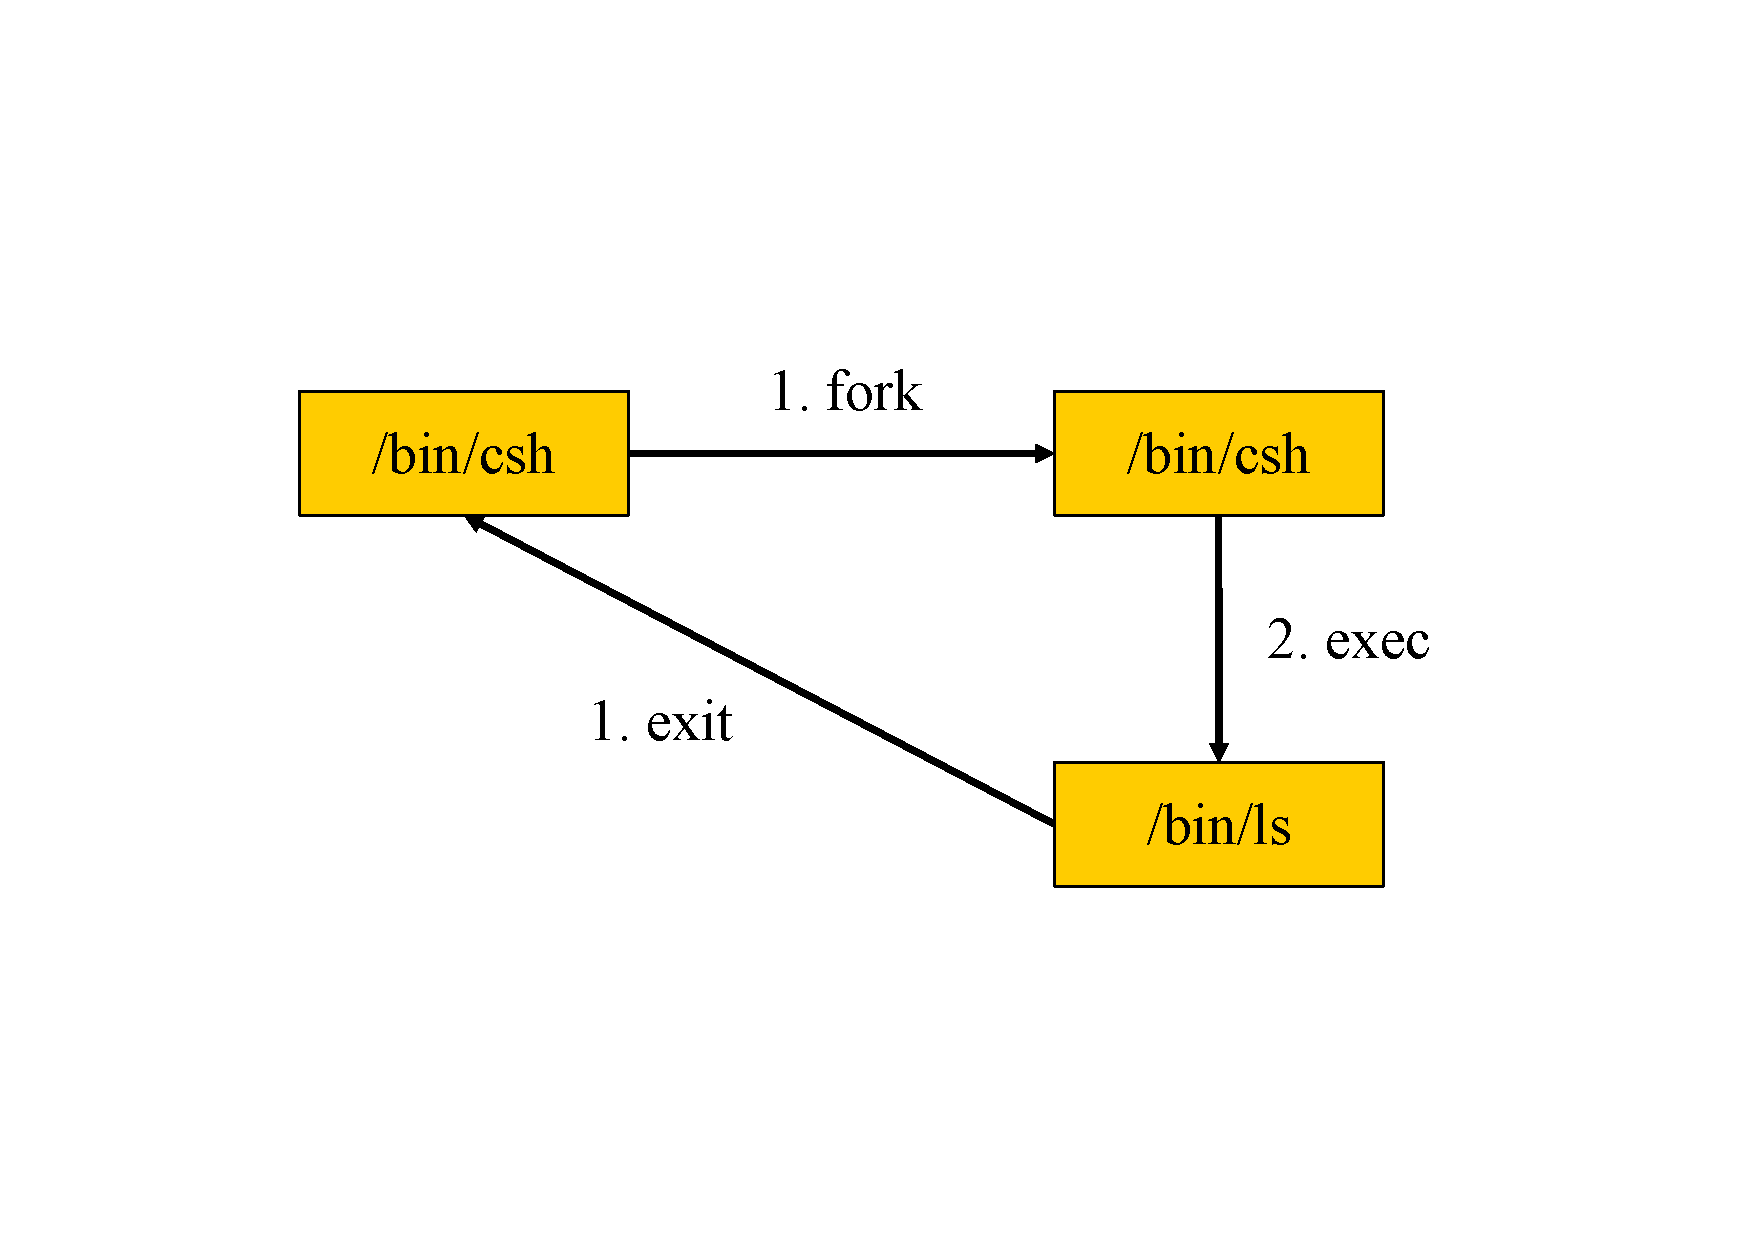
\includegraphics[height=5cm]{../illustration/execution_exemple.pdf}
\end{frame}


\begin{frame}
\frametitle{La primitive \texttt{exit()}}
\begin{itemize}
\item Quand un processus se termine
\begin{itemize}
\item Appel à la primitive \texttt{exit(status)}
\item Passe une information d’état au processus père
\end{itemize}
\item Un processus qui se termine :
\begin{itemize}
\item[1] Passe dans un état ``zombie''
\item[2] Attend que son père récupère son code retour par un \texttt{wait()}
\item[3] Il disparaît alors
\end{itemize}
\end{itemize}
\end{frame}


\begin{frame}
\frametitle{La primitive \texttt{wait()}}
\begin{itemize}
\item<1> Utilisée par un processus père 
\item<1> Récupère des informations d’un de ses fils venant de se terminer
\begin{itemize}
\item ``pid'' du processus fils venant de se terminer (le premier)
\item Contenu de la variable ``status''
\item Défini lors de l'appel à \texttt{exit()}
\end{itemize}
\item <2>Si le père se termine avant son fils
\begin{itemize}
\item Soit celui-ci est adopté par le processus "init"
\item Soit les fils sont terminés en cascade
\end{itemize}
\end{itemize}
\end{frame}

\begin{frame}
\frametitle{La primitive \texttt{wait()}}
\begin{columns}
\column{.6\textwidth}
\begin{small}
\verbatiminput{include/wait.c}
\end{small}
\column{.4\textwidth}
\begin{block}<only@2->{Exécution}
\begin{tiny}
Exemple d'utilisation de la fonction \texttt{wait()}

retour=    0 $\rightarrow$ a=0

retour=    0 $\rightarrow$ a=1

retour=    0 $\rightarrow$ a=2

retour=    0 $\rightarrow$ a=3

retour=    0 $\rightarrow$ a=4

En fin de compte, retour=0, a=5

retour=15330 $\rightarrow$ a=0

retour=15330 $\rightarrow$ a=1

retour=15330 $\rightarrow$ a=2

retour=15330 $\rightarrow$ a=3

retour=15330 $\rightarrow$ a=4

En fin de compte, pid=15330, a=5
\end{tiny}
\end{block}
\end{columns}
\end{frame}

\begin{frame}
\frametitle{La primitive \texttt{waitpid()}}
\begin{itemize}
\item Permet d'attendre la fin d'un processus particulier
\item Syntaxe :
\begin{itemize}
\item \texttt{waitpid(int pid, int *status, int option)}
\item l'option est 0 en général, ou WNOHANG. ce code est une version non bloquante de wait. 
\end{itemize}
\end{itemize}
\end{frame}



\subsection{Espace d’adressage séparé}

\begin{frame}{Espace d’adressage séparé}
\begin{itemize}
\item Processus indépendants
\begin{itemize}
\item exécution indépendante des autres processus
\item ne doit pas perturber les autre processus
\item ne doit pas être impacté par les autres processus
\end{itemize}
\item Protection de l'espace d'adressage 
\begin{itemize}
\item vis à vis des autres processus
\item contre ses propres débordements
\end{itemize}

\item Espace d'adressage dédié 
\begin{itemize}
\item cloisonnement de l'espace mémoire
\item adressage local
\item le reste de la mémoire l'existe pas
\end{itemize}
\end{itemize}
\end{frame}


\section{Parallélisme et programmation concurrente}

\subsection{Ordonnancement de processus}

\begin{frame}
\frametitle{Ordonnancement de processus}
\begin{itemize}
\item Nécessaire à l’utilisation efficace des ressources
\begin{itemize}
\item la quasi totalité des ressources est ordonnancée
\end{itemize}
\item Gestion de la concurrence inter-processus
\begin{itemize}
\item accès à la CPU
\item accès aux périphériques
\end{itemize}
\item Commutations rapides
\begin{itemize}
\item illusion d’une exécution simultanée
\end{itemize}
\end{itemize}
\end{frame}


\begin{frame}
\frametitle{Les trois niveaux d'ordonnancement}
\begin{itemize}
\item Ordonnancement à \textbf{long terme}
\begin{itemize}
\item Choix des travaux à entreprendre
\item Contrôle le degré de multiprogrammation
\item Long et peu fréquent
\end{itemize}
\item Ordonnancement à \textbf{moyen terme}
\begin{itemize}
\item Permutation swapping
\end{itemize}
\item Ordonnancement à \textbf{court terme} (exécution)
\begin{itemize}
\item Choix des processus à exécuter
\item Rapide et fréquent
\end{itemize}
\end{itemize}
\end{frame}


\begin{frame}
\frametitle{La commande \texttt{ps} d'Unix}
\begin{itemize}
\item Liste des processus avec leur état
\begin{center}
\verbatiminput{include/ps.txt}
\end{center}
\item Runing, sTopped, Sleeping ($\leq$20s), Idle ($\succ$20s), P : en attente de page, D : en attente d'une E/S disque
\item W : swappé, Zombie, ``rien'' : en mémoire
\end{itemize}
\end{frame}


\begin{frame}
 \framesubtitle{Ordonnancement à moyen terme}
 \frametitle{Permutation swapping \cite{pase}}
 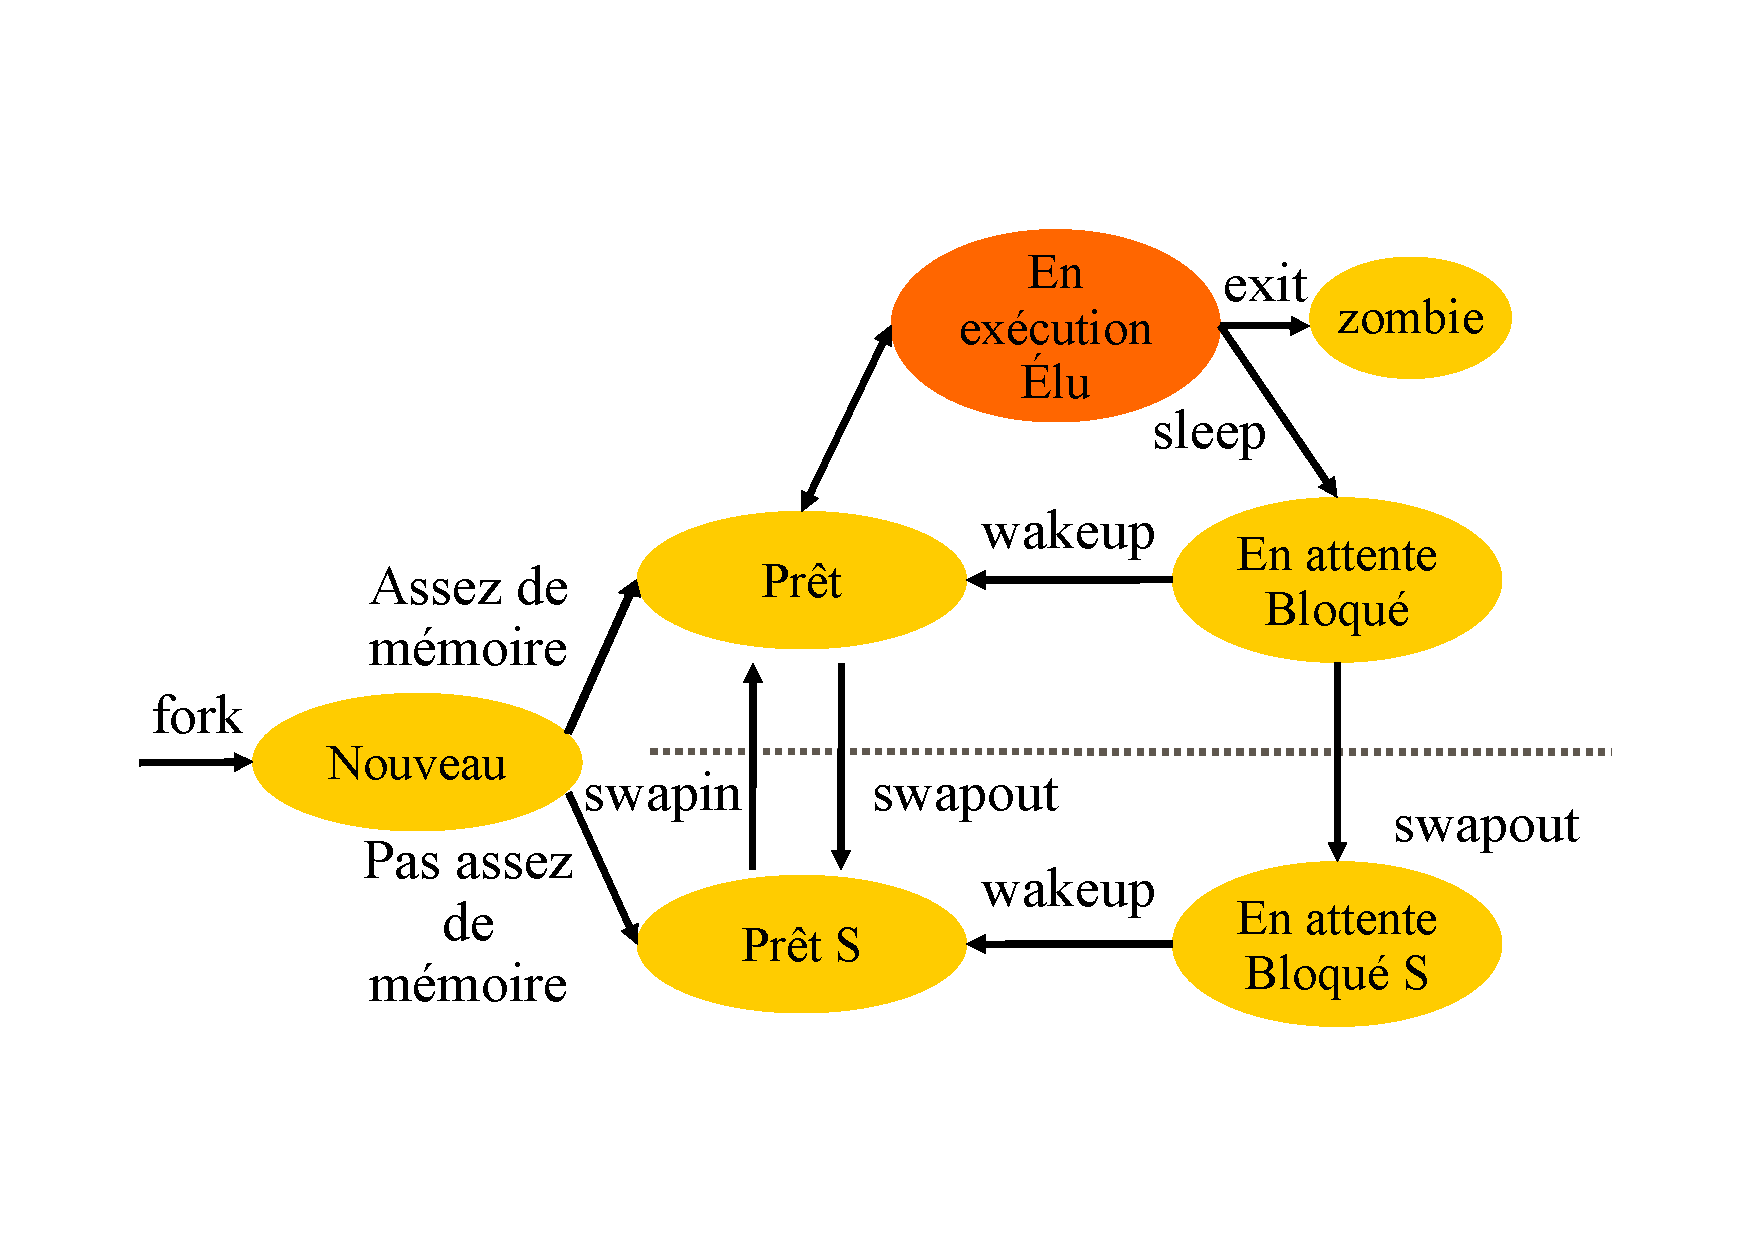
\includegraphics[width=.8\textwidth]{../illustration/permut_swap_cycle_vie.pdf}
\end{frame}


\begin{frame}
 \frametitle{Exécution - runtime}
 \framesubtitle{Ordonnancement à court terme}
 
 \begin{center}
 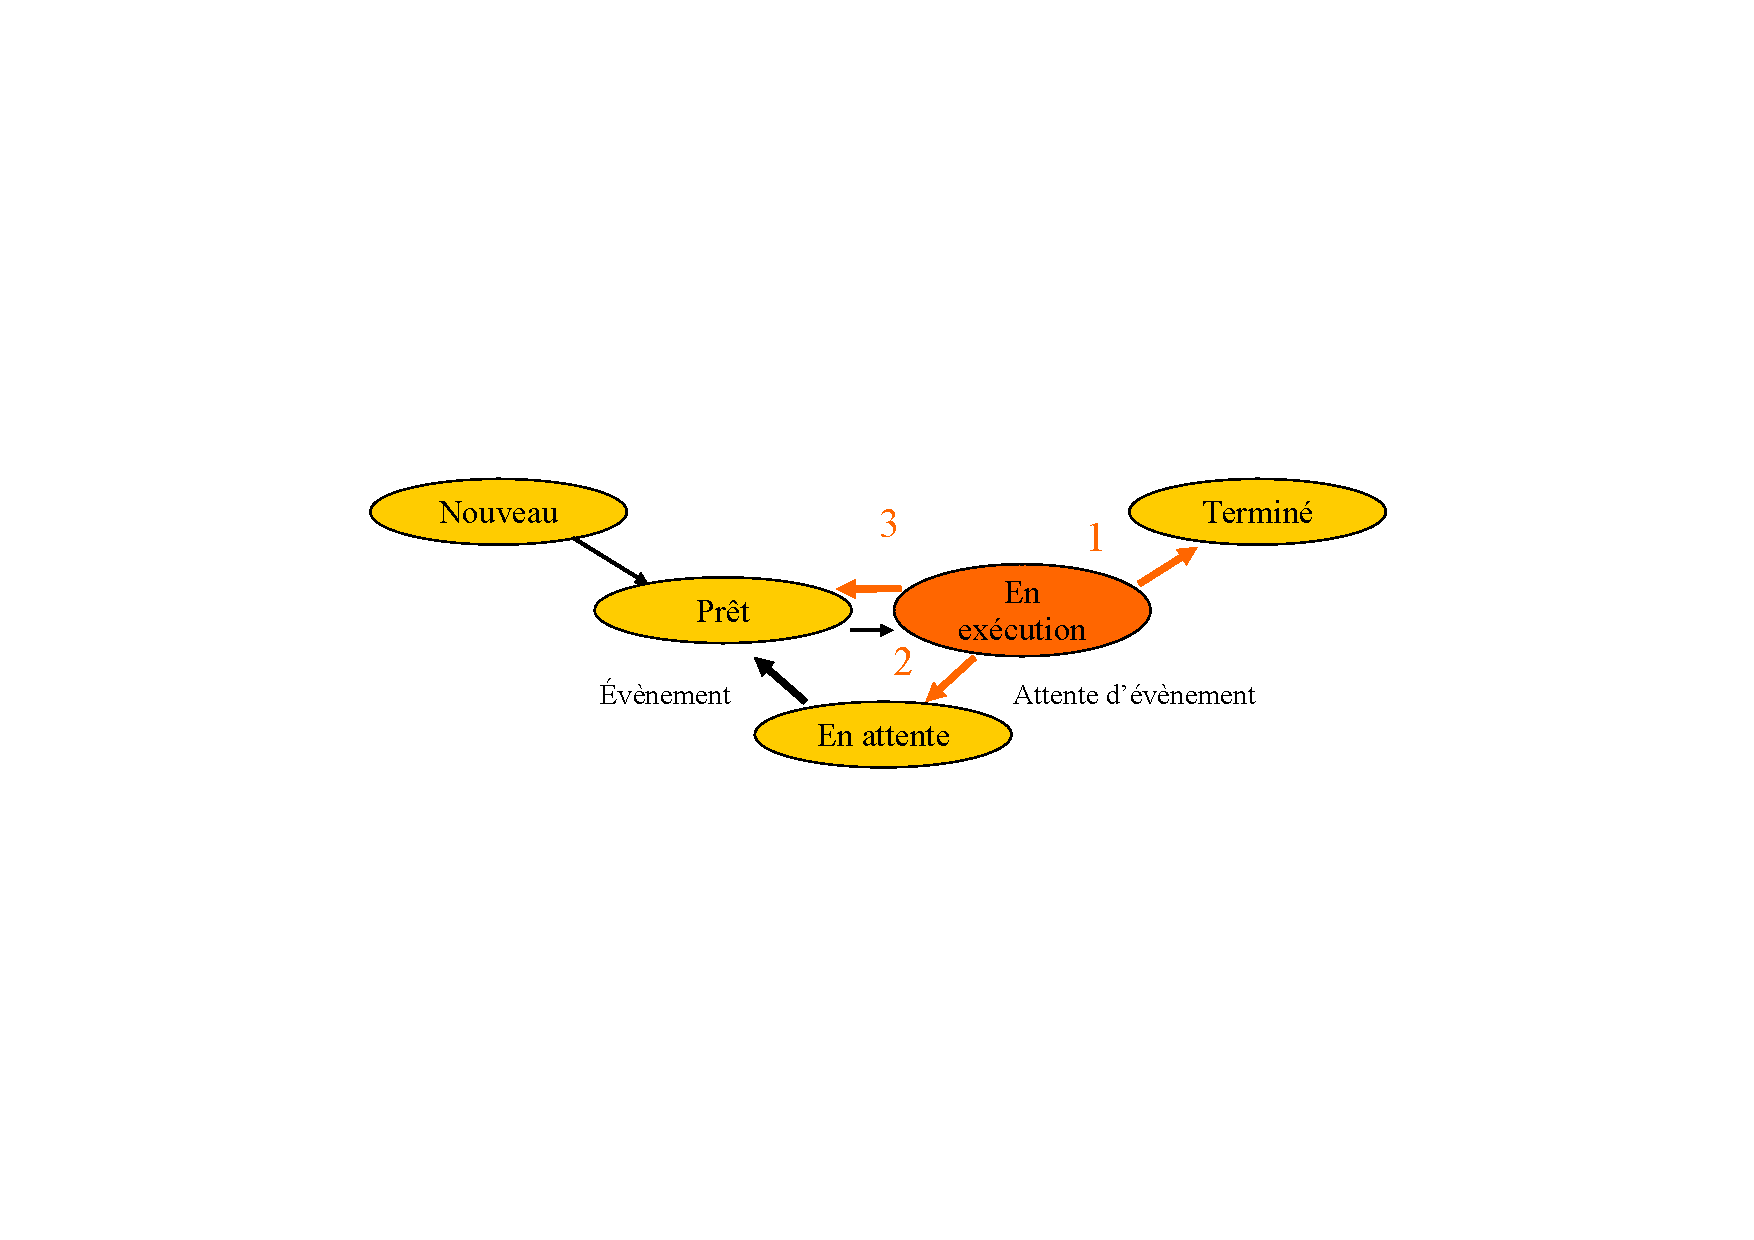
\includegraphics[height=3cm]{../illustration/cycle_court_terme.pdf}
 \end{center}
 \begin{itemize}
 \item Cas 1 et 2 : non préemptif (coopératif)
 \item Cas 3 : préemptif
 \end{itemize}
\end{frame}



\begin{frame}
 \frametitle{Le dispatcheur}
 \begin{itemize}
 \item Elément central du système
 \item Donne le contrôle de la CPU au processus choisi par l’ordonnanceur à court terme
\begin{itemize}
\item sauvegarde PSW processus sortant
\item restauration PSW processus entrant
\item mise à jour des PCB
\end{itemize}
\item Latence du dispatcheur
	\begin{itemize}
\item temps pris par le dispatcheur pour stopper un processus et (re)lancer un autre 
\end{itemize}

 \end{itemize}
\end{frame}


\begin{frame}
 \frametitle{Critères d’ordonnancement}
 \begin{itemize}
 \item Utilisation CPU (\%)
 \begin{itemize}
 \item La plus élevée possible
 \end{itemize}
 \item Débit 
 \begin{itemize}
 \item Nombre de processus terminés par seconde
 \end{itemize}
 \item Temps :
\begin{itemize}
\item de rotation
\item d’attente
\item de réponse
\end{itemize}

\end{itemize}
\end{frame}

\begin{frame}
 \frametitle{Cycle UC et cycle E/S}
 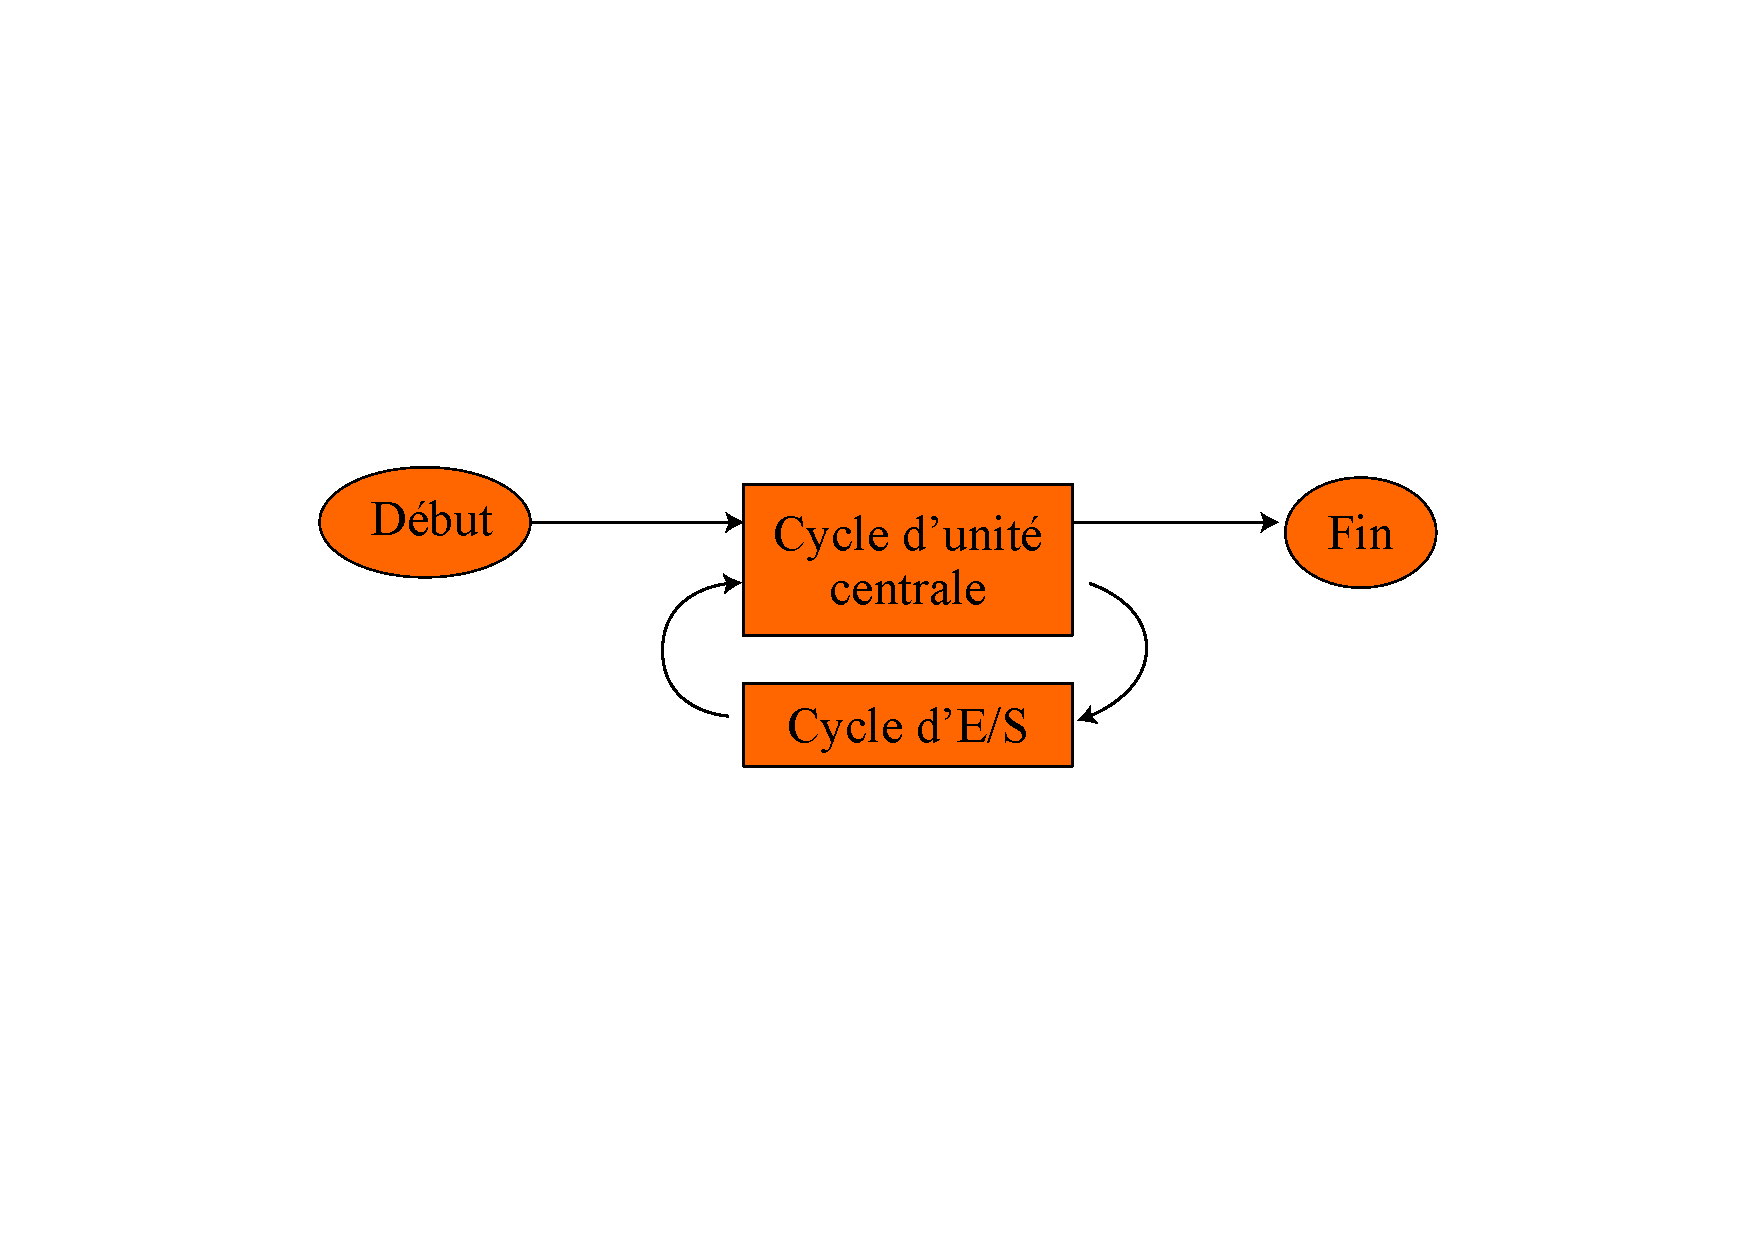
\includegraphics[width=.9\textwidth]{../illustration/cycle_es_uc.pdf}
 \begin{itemize}
 \item Deux familles de processus :
 \begin{itemize}
 \item Tributaires de l’UC (calculs)
 \item Interactifs et tributaires des E/S
 \end{itemize}
 \item Répartition importante pour les choix d’algorithme d’ordonnancement
 \end{itemize}
\end{frame}



\begin{frame}
 \frametitle{Files d’attente d’ordonnancement}
 \begin{itemize}
 \item Outil de travail de l'ordonnanceur
 \item Listes chaînées de PCB
 \begin{itemize}
 \item Nouveaux processus :
 \begin{itemize}
 \item File d’attente des travaux
 \end{itemize}
 \item Processus prêts :
 \begin{itemize}
 \item File d’attente des processus prêts
 \end{itemize}
 \item Processus bloqués :
 \begin{itemize}
 \item Liste d’attente de périphériques
 \end{itemize}
 \end{itemize}
 \item Mise à jour atomiques
\begin{itemize}
 \item Temps réel
 \item Multi-processeur
 \end{itemize}
 \end{itemize}
\end{frame}

\begin{frame}
 \frametitle{Exemples de files d’attente}
 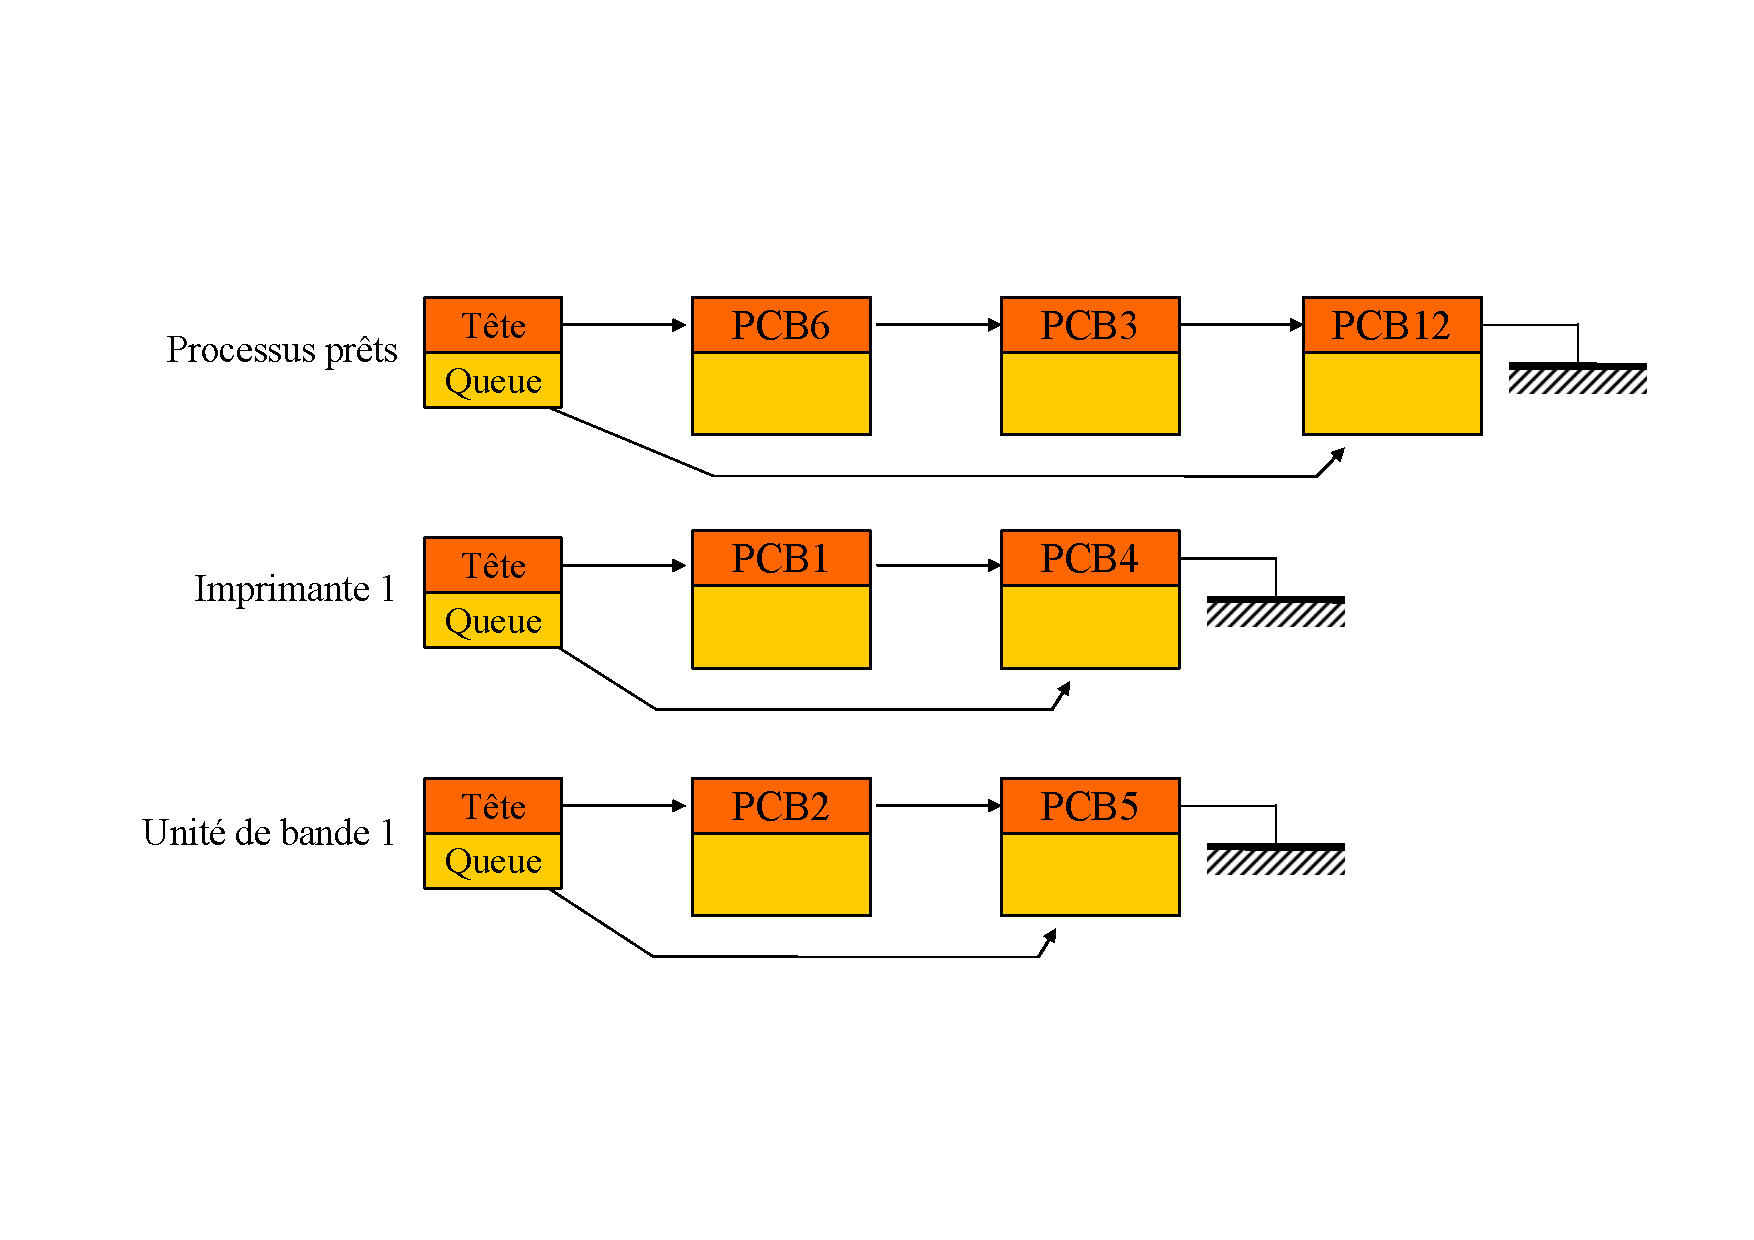
\includegraphics[width=\textwidth]{../illustration/exemple_file_attente.pdf}
\end{frame}


\begin{frame}
 \frametitle{Diagramme des files d’attente}
 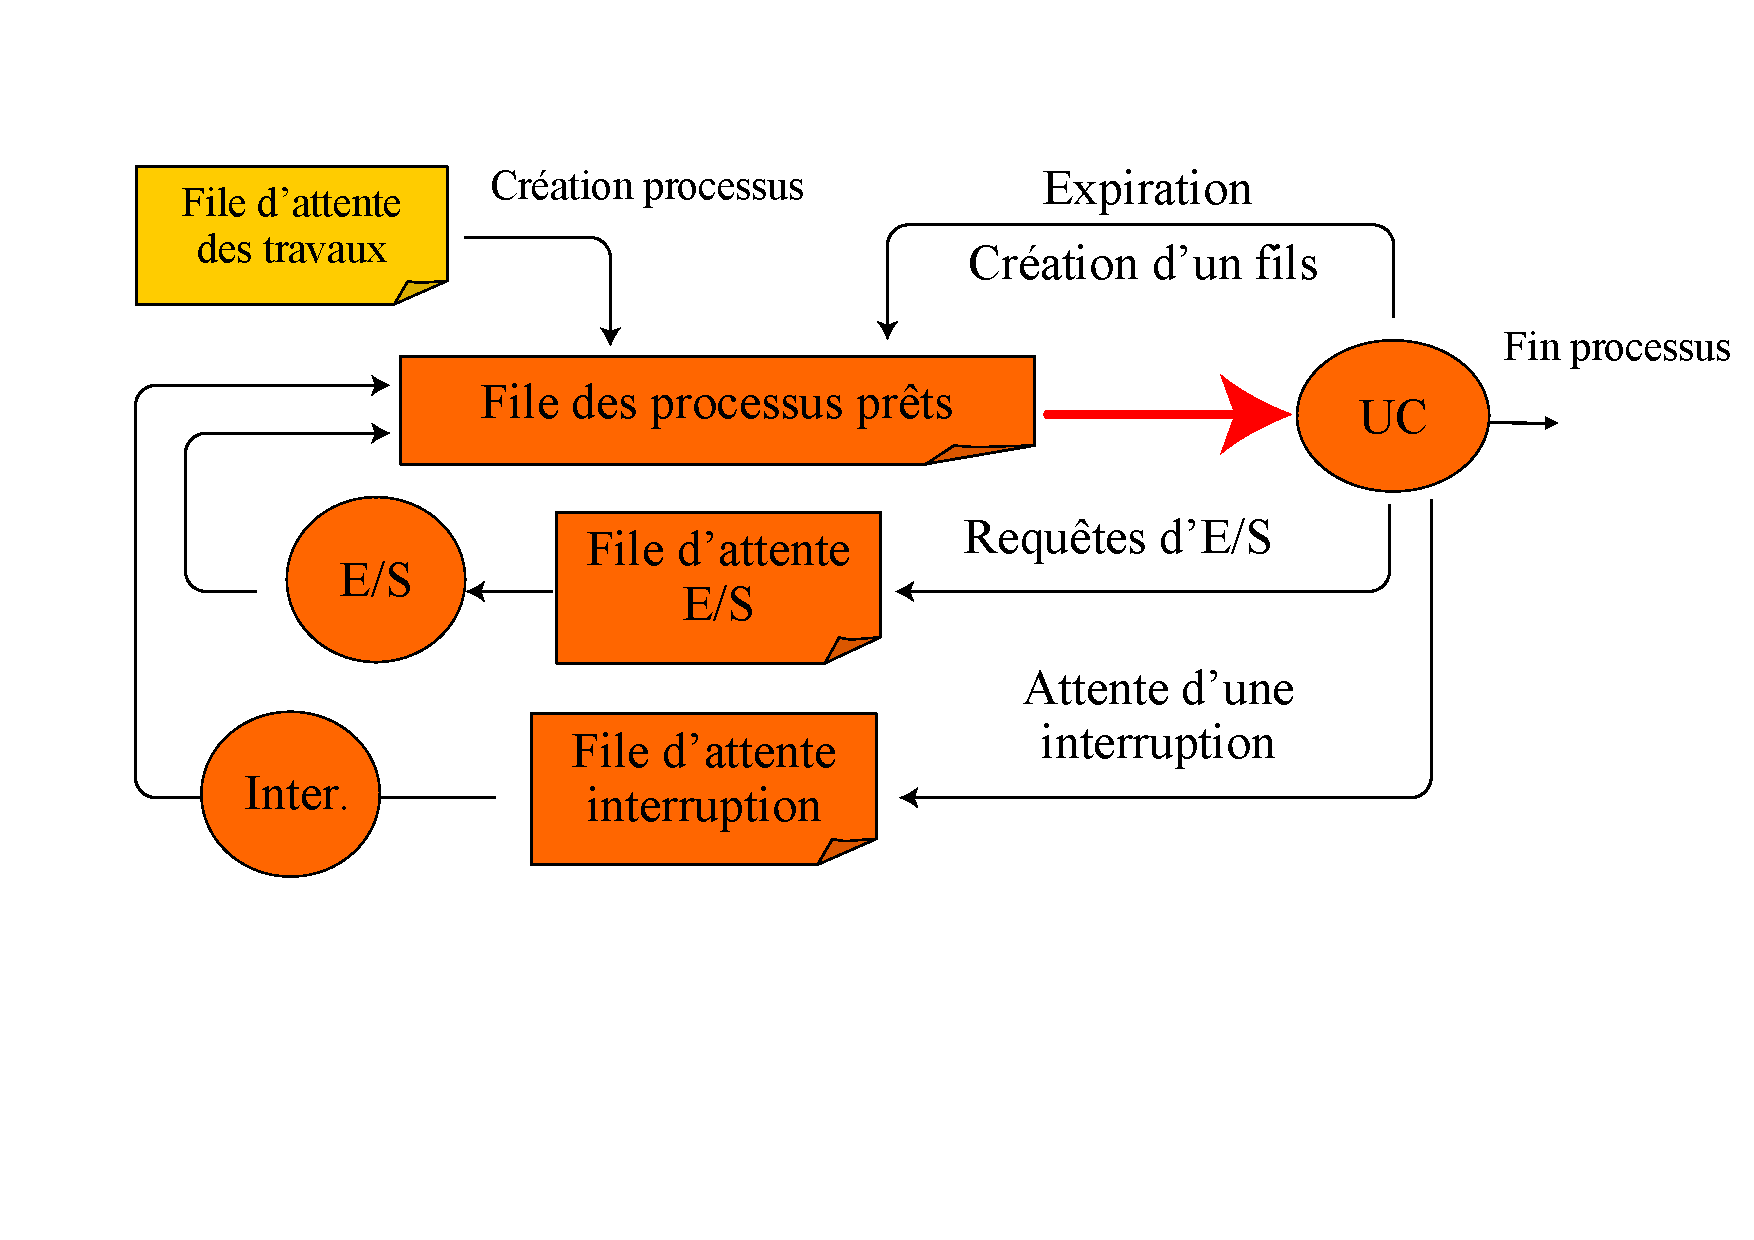
\includegraphics[width=\textwidth]{../illustration/diag_file_attente.pdf}
\end{frame}


\subsection{Algorithmes d'ordonnancement}

\begin{frame}
 \frametitle{Algorithmes d’ordonnancement}
 \begin{itemize}
 \item Premier arrivé premier servi (FCFS)
 \item Plus court travail d’abord (SJF)
 \item Tourniquet (RR)
 \item Multi niveau
 \item Multi niveau à retour
 \item Multi processeurs
 \item Temps réel
\end{itemize}
\end{frame}



\begin{frame}
 \frametitle{Premier arrivé, premier servi : FCFS}
 \begin{itemize}
 \item Simple
 \begin{itemize}
 \item File d’attente FIFO
 \end{itemize}
 \item Temps d’attente moyen
 \begin{itemize}
 \item Long
 \item Très variable
 \end{itemize}
 \item Effet d’accumulation
 \end{itemize}
\end{frame}


\begin{frame}
 \frametitle{Exemple FCFS}
 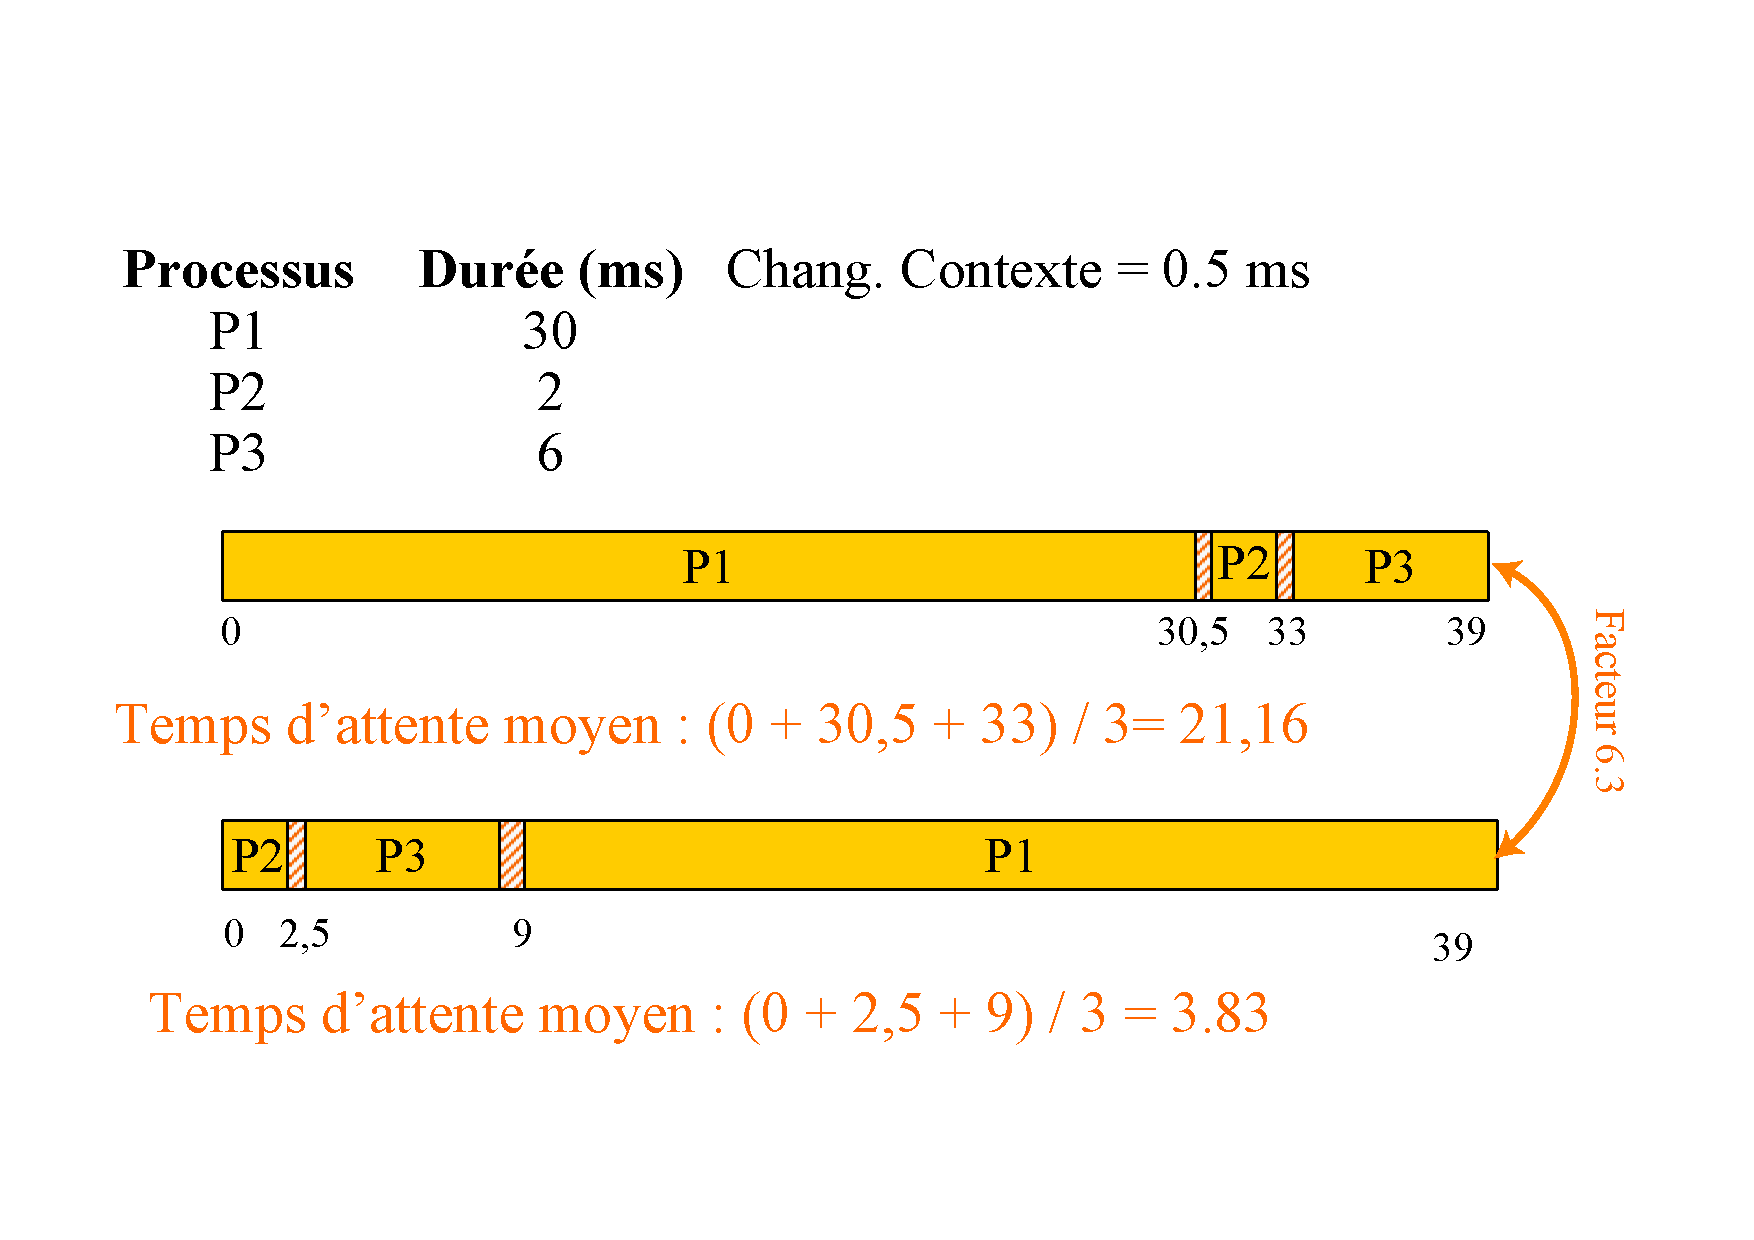
\includegraphics[width=\textwidth]{../illustration/fcfs_exemple.pdf}
\end{frame}


\begin{frame}
 \frametitle{Travail le plus court d’abord : SJF}
 \begin{itemize}
 \item Nécessite de connaître la durée du prochain cycle d’exécution
\begin{itemize}
 \item Difficulté d’estimation
 \begin{itemize}
 \item indications de l’utilisateur
 \item moyenne exponentielle des durées cycles précédents 
 \end{itemize}
 \end{itemize}

 \item Optimise le temps d’attente moyen
\item Difficile à mettre en oeuvre
 \end{itemize}
\end{frame}



\begin{frame}
 \frametitle{Ordonnancement avec priorité}
 \begin{itemize}
 \item Priorité sur chaque processus
 \begin{itemize}
 \item en fonction de contraintes
 \begin{itemize}
 \item internes (besoin mémoire, rapport CPU/ES...)
 \item externes (type travail, contrat, politique... )
 \end{itemize} \end{itemize}

 
 \item Processus traités par ordre de priorité suivant FCFS
 \begin{itemize} \item préemptif ou non  \end{itemize}
 \item Famine (blocage infini) $\rightarrow$ vieillissement
 \end{itemize}
\end{frame}



\begin{frame}
 \frametitle{Ordonnancement à tourniquet : RR (round robin)}
 \begin{itemize}
 \item Quantum de temps\footnote{Fixé à 60ms, par exemple}
 \begin{itemize}
\item Registre horloge (RH ou RTempo)
\item PIT : Programmable Interrupt Timer
\item Si RH = 0 : interruption d'horloge (ITH)
\end{itemize}

 \item File des processus prêts circulaire
 \item Temps d’attente lié au quantum
 \begin{itemize}
 \item Quantum faible $\rightarrow$ partage de l’UC
 \item Quantum grand $\rightarrow$ FCFS
 \item Surcoût du changement de contexte
 \end{itemize}
 \end{itemize}
\end{frame}


\begin{frame}
 \frametitle{Exemple RR}
 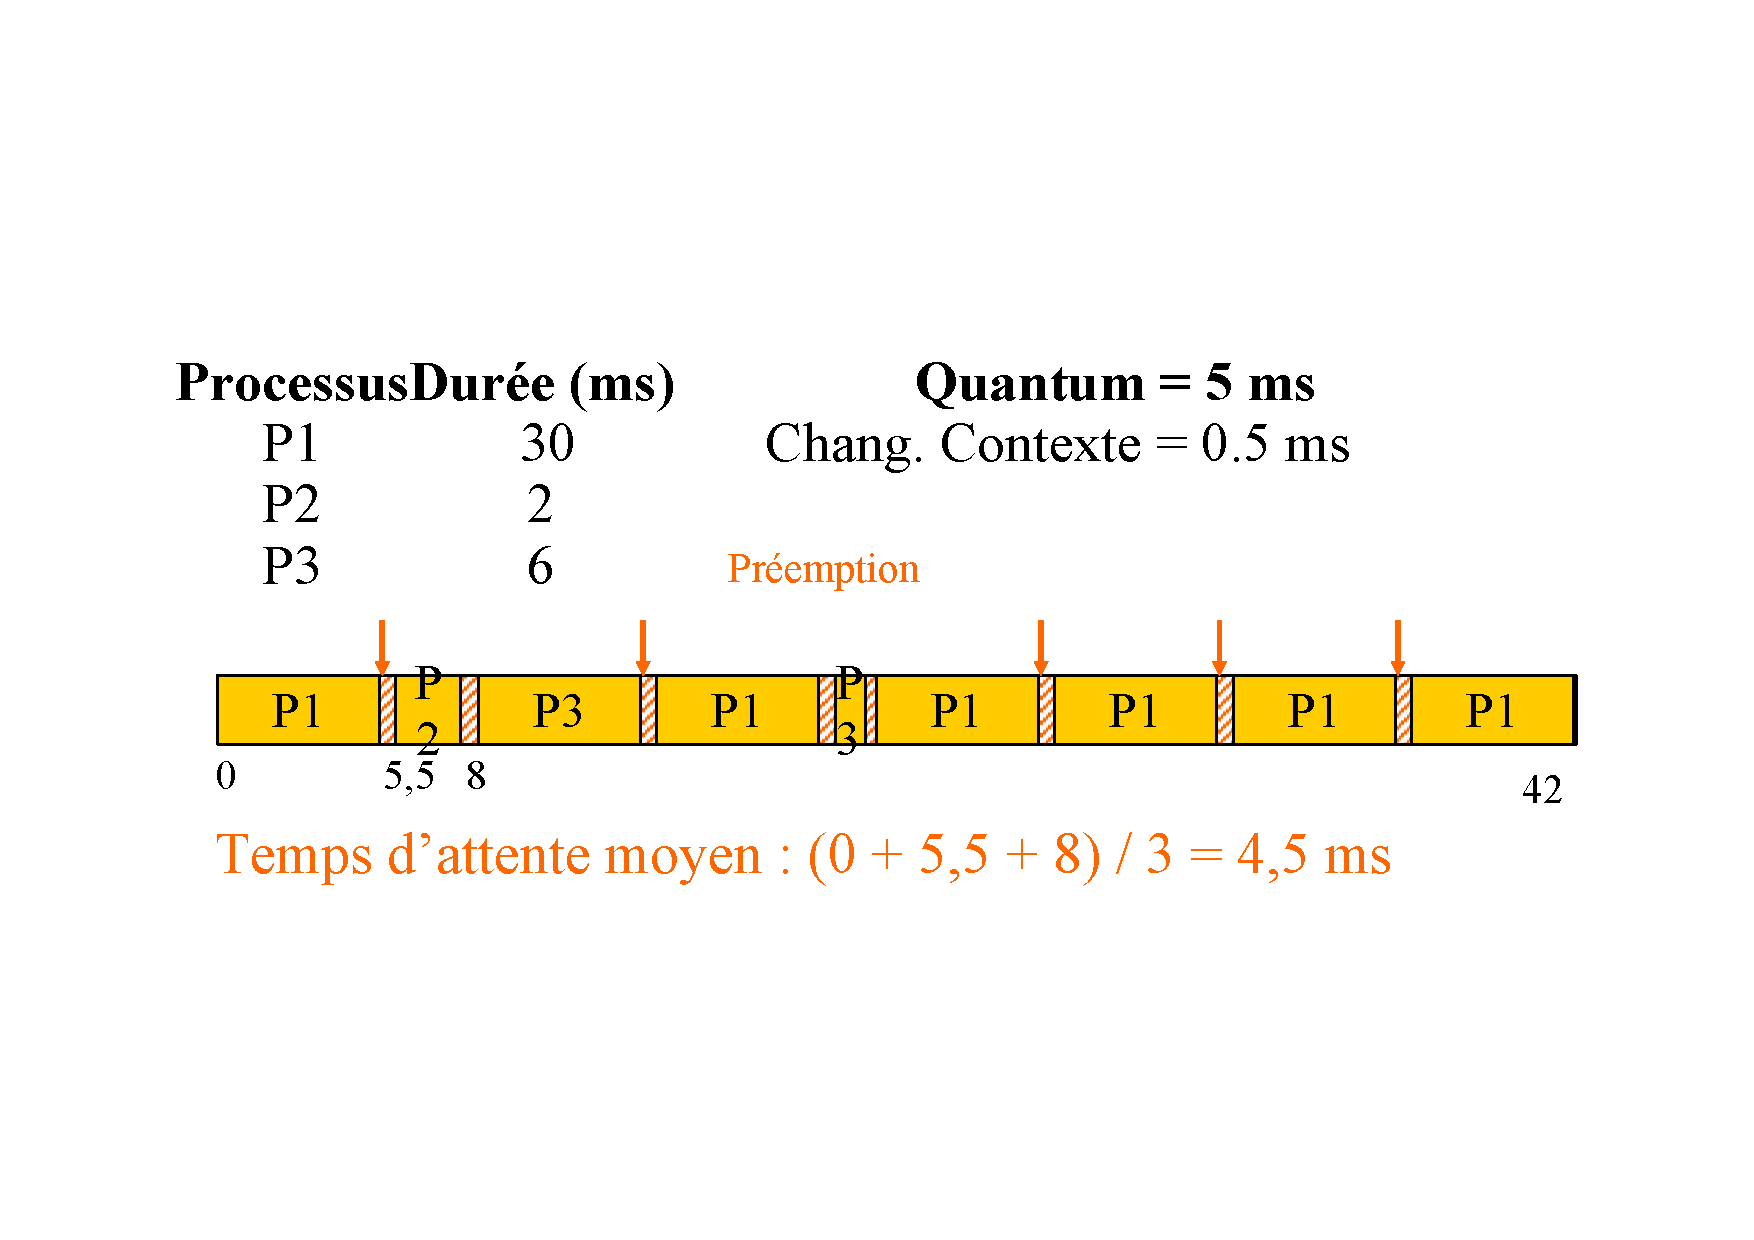
\includegraphics[width=\textwidth]{../illustration/rr_exemple.pdf}
\end{frame}

\begin{frame}
\frametitle{Ordonnancement par loterie}
\begin{itemize}
\item Principe :
\begin{itemize}
\item Distribution de "tickets" (CPU, mémoire...)
\item Tirage du gagnant à intervalle fixe
\item ...jusqu'à épuisement des tickets distribués.
\end{itemize}
\item Avantages :
\begin{itemize}
\item Mécanisme de promesse
\item Partage équitable des ressources (garanti)
\end{itemize}

\end{itemize}
\end{frame}



\begin{frame}
 \frametitle{Ordonnancement à files multi niveau}
 \begin{itemize}
 \item Classement des travaux en groupes
 \begin{itemize}
 \item Exemple : Interactif et arrière plan (lots)
 \item Plusieurs files d’attente
 \end{itemize}
 \item Algorithme d’ordon. propre à chaque file
 \begin{itemize}
 \item Exemple : interactif $\rightarrow$ RR et lots $\rightarrow$ FCFS
 \end{itemize}
 \item Priorité entre listes
 \begin{itemize}
 \item Exploite une file lorsque toutes les files de niveau supérieur sont vides
 \end{itemize}
 \end{itemize}
\end{frame}


\begin{frame}
 \frametitle{Ordonnancement avec files multi niveau à retour}
 \begin{itemize}
 \item Multi niveau + déplacement entre files
 \item Caractérisé par :
 \begin{itemize}
 \item Nombre de files
 \item Algorithme d’ordonnancement de chaque file
 \item Méthode de déplacement entre files
 \item File d’entrée
 \end{itemize}
 \item Général et configurable à souhait
 \end{itemize}
\end{frame}


\begin{frame}
 \frametitle{Ordonnancement avec files multi niveau à retour}
 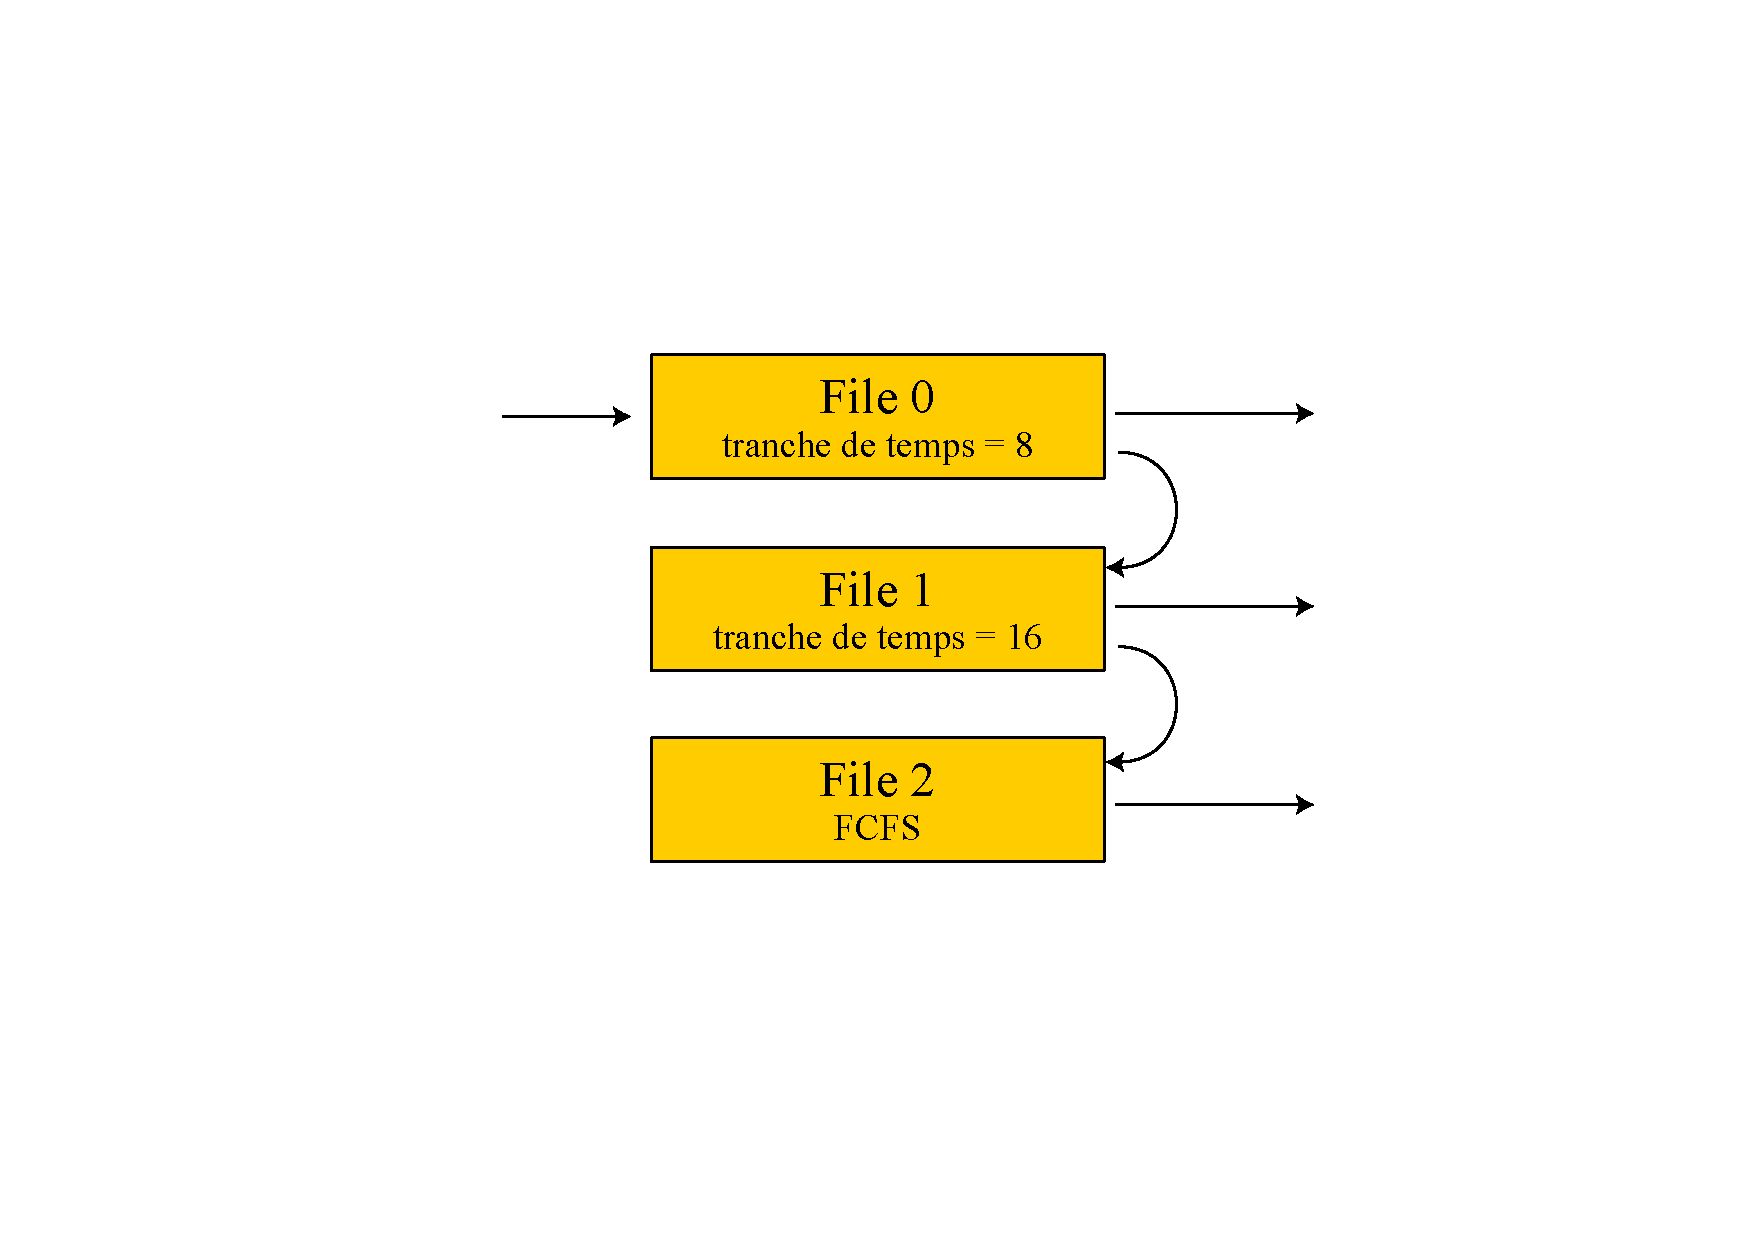
\includegraphics[width=.8\textwidth]{../illustration/multiniveau_retour.pdf}
\end{frame}



\begin{frame}
 \frametitle{Ordonnancement multi processeurs}
 \begin{itemize}
  \item Partage de charge entre les processeurs 
  \item File d’attente commune
  \item Deux approches :
  \begin{itemize}
   \item Multitraitement \textbf{symétrique} (SMP)
   \begin{itemize}
    \item Ordonnancement indépendant pour chaque CPU
   \end{itemize}
   \item Multitraitement \textbf{asymétrique} (AMP)
   \begin{itemize}
    \item Ordonnancement centralisé (CPU maître)
    \item Distribution des processus sur les autres CPU (mode utilisateur)
   \end{itemize}
  \end{itemize}
 \end{itemize}
\end{frame}


\begin{frame}
 \frametitle{Ordonnancement temps réel rigide}
 \begin{itemize}
 \item Contrainte : délai garanti
 \begin{itemize}
 \item Temps nécessaire indiqué lors de la soumission
 \item Travail admis ou rejeté par le système
 \end{itemize}
 \item Temps de réponse des E/S constants
 \begin{itemize}
 \item Réservation de ressources à l'avance
 \end{itemize}
 \item Matériel et un système souvent dédiés
 \end{itemize}
\end{frame}

\begin{frame}
 \frametitle{Ordonnancement temps réel souple}
 \begin{itemize}
 \item Temps de dispatch faible
 \item Processus temps réel
 \begin{itemize}
  \item Priorité la plus haute
  \item Héritage de priorité
 \end{itemize}
 \item Problème des appels système
 \begin{itemize}
  \item Points de reprise réguliers
  \item Noyau préemptable (protection structures)
 \end{itemize}
 \end{itemize}
\end{frame}



\subsection{Les threads}

\begin{frame}
 \frametitle{Principe des threads}
 \begin{itemize}
 \item Jusqu’à présent :
 \begin{itemize}
 \item 1 processus = 1 programme en exécution
 \item Flot de contrôle (thread) unique
 \end{itemize}
 \item Processus multi-thread
 \begin{itemize}
 \item Flots de contrôle multiples
 \begin{itemize}
 \item fils d’exécution indépendants
 \end{itemize}
 \item Peut effectuer plusieurs tâches simultanées au sein d’un même processus
 \end{itemize}
 \item Géré par les OS récents
 \end{itemize}
\end{frame}


\begin{frame}
 \frametitle{Principe des threads}
 \begin{itemize}
 \item Les différents threads d’un processus :
 \begin{itemize}
 \item Même espace d'adressage en mémoire
 \item Exécution concurrente
\end{itemize}
\item Collaboration facilitée
\begin{itemize}
 \item Partage du code exécutable
 \item Accès au même contenu de la mémoire
 \item Utilisation de ressources communes
 \end{itemize}
 \item Facilité de mise en oeuvre de traitements parallèles
 \end{itemize}
\end{frame}



\begin{frame}
 \frametitle{Processus concurrents}
 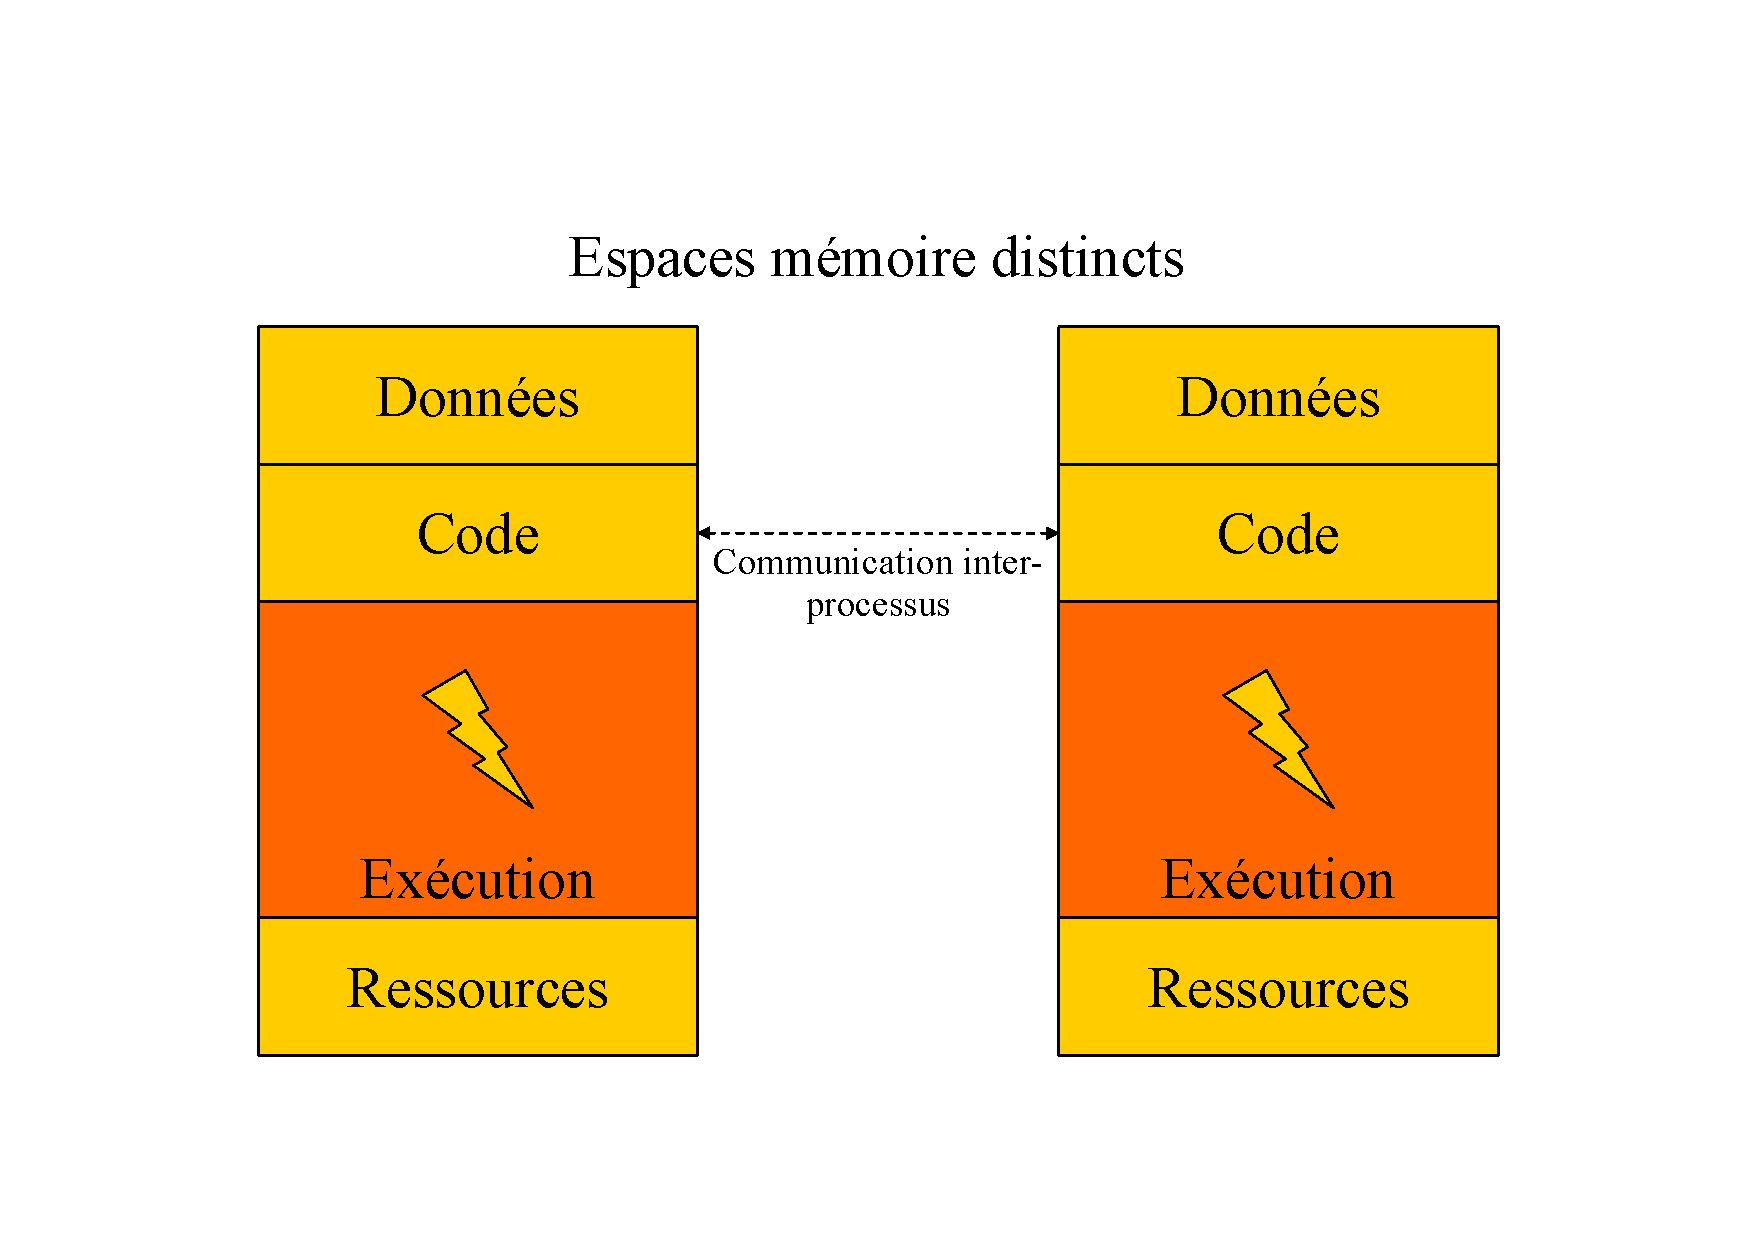
\includegraphics[width=.8\textwidth]{../illustration/processus_concurrents.pdf}
\end{frame}


\begin{frame}
 \frametitle{Processus multi-thread}
 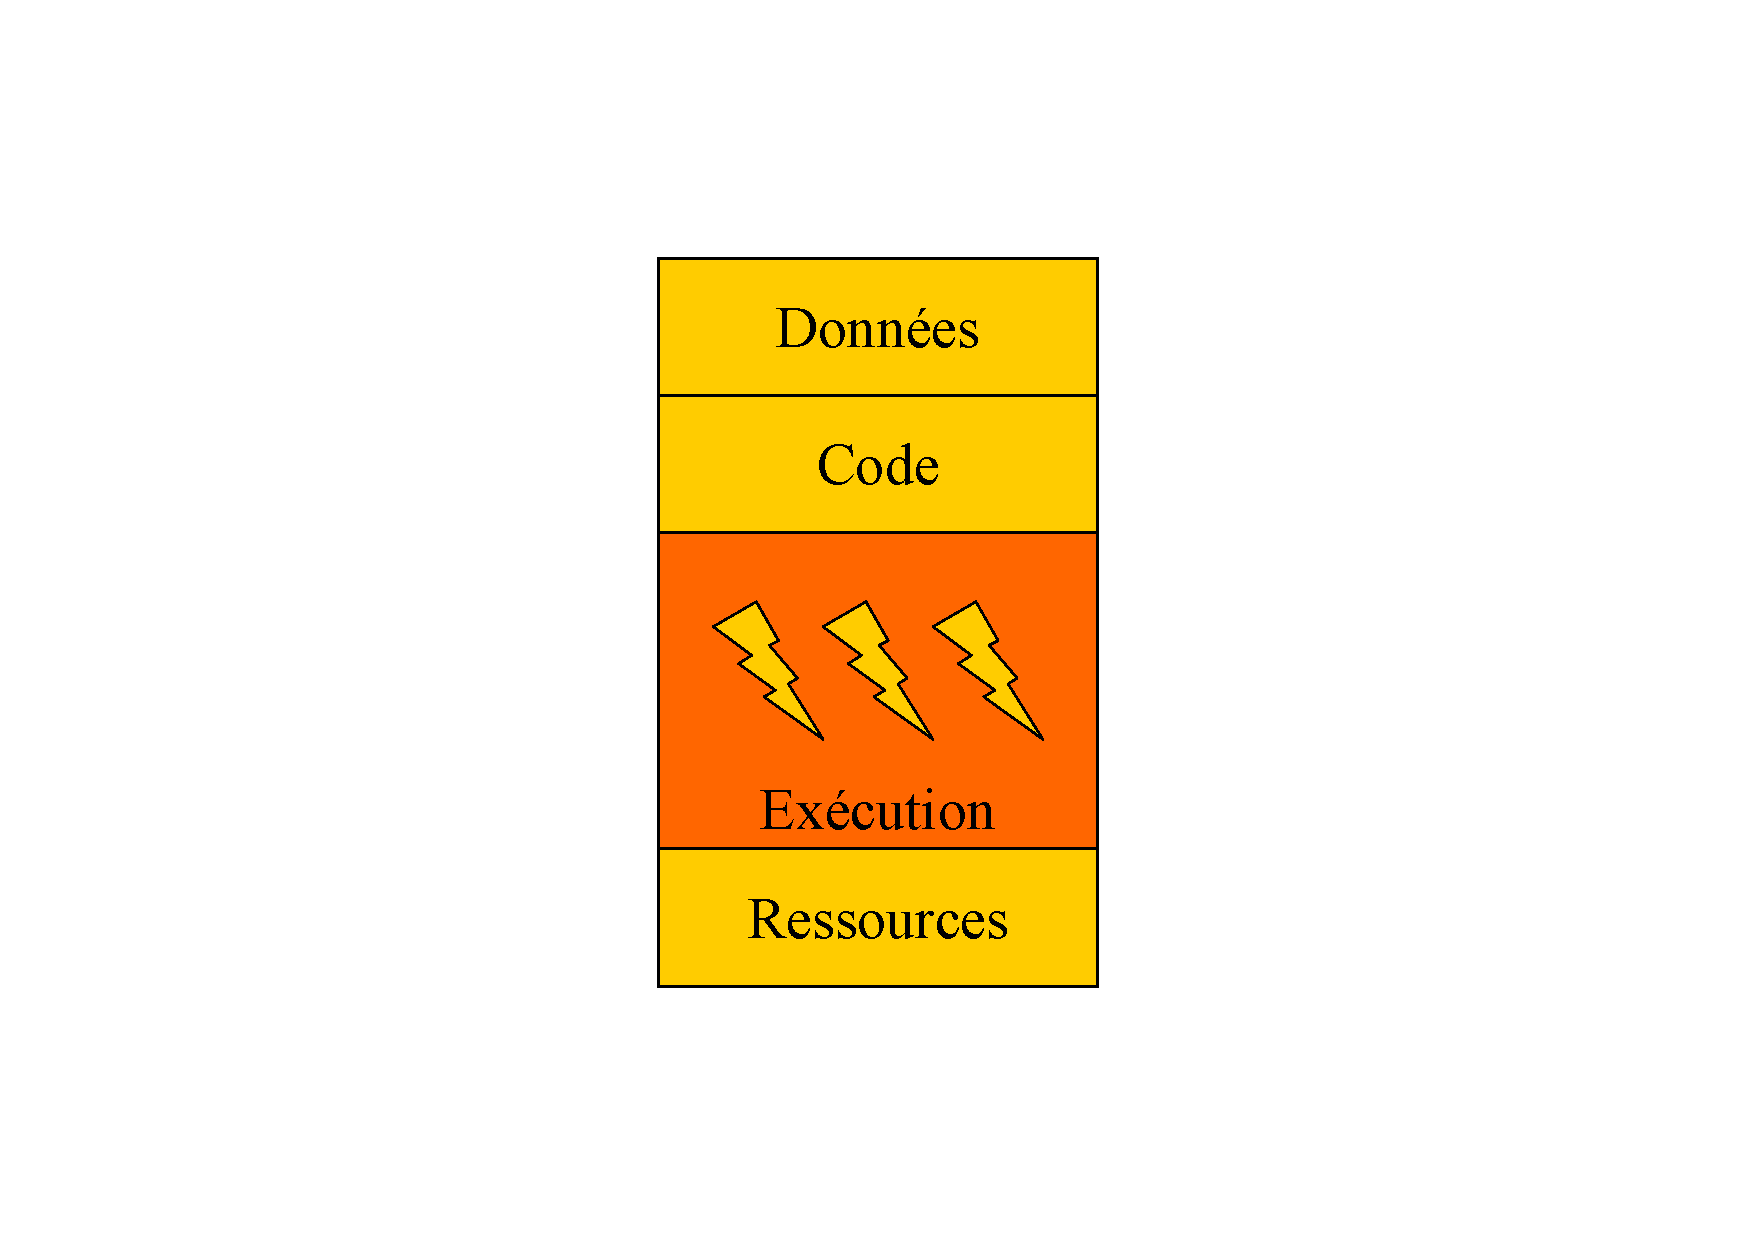
\includegraphics[width=.5\textheight]{../illustration/processus_multithread.pdf}
\end{frame}


\begin{frame}
 \frametitle{Composition d’un processus multi-thread}
 \begin{itemize}
 \item Commun à tous les flots du processus :
 \begin{itemize}
 \item Code
 \item Données
 \item Ressources (fichiers, signaux)
 \end{itemize}
 \item Propre à chaque flot :
 \begin{itemize}
 \item Identificateur de thread
 \item Compteur programme (compteur ordinal)
 \item Registres
 \item Pile
 \end{itemize}
 \end{itemize}
\end{frame}


\begin{frame}
 \frametitle{Thread = processus léger}
 \begin{itemize}
 \item Fonctionnement asynchrone au sein d’un même processus
 \item Moins coûteux à créer qu’un processus
 \item Éventuellement moins coûteux à ordonnancer
 \end{itemize}
\end{frame}


\begin{frame}
 \frametitle{Avantages du processus léger}
 \begin{itemize}
 \item Réactivité
 \begin{itemize}
 \item Maintient de l’interactivité au sein d’un processus
 \end{itemize}
 \item Partage de ressource
 \begin{itemize}
 \item Partage mémoire et code (espace d’adressage)
 \end{itemize}
 \item Économie
 \begin{itemize}
 \item Ressources partagées (mémoire, fichiers… )
 \item Gestion, ordonnancement
 \end{itemize}
 \end{itemize}
\end{frame}


\begin{frame}
 \frametitle{Les deux types de threads}
 \begin{columns}
 \column{.5\textwidth}
 \begin{block}{Thread utilisateur}
 \begin{itemize}
 \item Utilisé dans les programmes utilisateur
 \item Manipulé au niveau utilisateur
 \end{itemize}
 \end{block}
 \column{.5\textwidth}
 \begin{block}{Thread système/noyau}
 \begin{itemize}
 \item Implémentés par le système
 \item Manipulés par des appels système
 \end{itemize}
 \end{block}
 \end{columns}
\end{frame}


\begin{frame}
 \frametitle{Thread utilisateur}
 \begin{itemize}
 \item Gestion des thread au niveau utilisateur
 \begin{itemize}
 \item Bibliothèque de gestion de thread
 \item Entité manipulée par le programmeur
 \item Parallélisation algorithmique
 \end{itemize}
 \end{itemize}


 \begin{exampleblock}{Exemples}
 \begin{itemize}
 \item POSIX
 \item C-threads Mach
 \item Light-weight process Solaris
 \item Threads Java
 \end{itemize}
 \end{exampleblock}
\end{frame}


\begin{frame}
 \frametitle{Thread noyau}
 \begin{itemize}
 \item Gestion des thread fournie par le système
 \begin{itemize}
 \item Pris en charge par le système
 \item Coût de création et de gestion
 \item Exploitation des architectures multiprocesseur
 \end{itemize}
 \end{itemize}
 \begin{exampleblock}{Exemples}
 \begin{itemize}
 \item Windows NT, Solaris, Linux...
 \item Threads natifs Java
 \end{itemize}
 \end{exampleblock}
\end{frame}

\subsection{Ordonnancement de thread}

\begin{frame}
 \frametitle{Ordonnancement de thread}
 \begin{itemize}
 \item Trois modèles de prise en charge :
 \begin{itemize}
 \item plusieurs vers un
 \item un vers un
 \item plusieurs vers plusieurs
 \end{itemize}
 \end{itemize}
\end{frame}


\begin{frame}
 \frametitle{Le modèle ``plusieurs vers un''}
 \begin{columns}
 \column{0.5\textwidth}
 \begin{itemize}
 \item Efficace (niveau utilisateur)
 \item Possibilité de blocage
 \item Pas de parallèlisation
 \item Utilisé par les OS ne supportant pas le multithreading
 \end{itemize}
 \column{0.5\textwidth}
 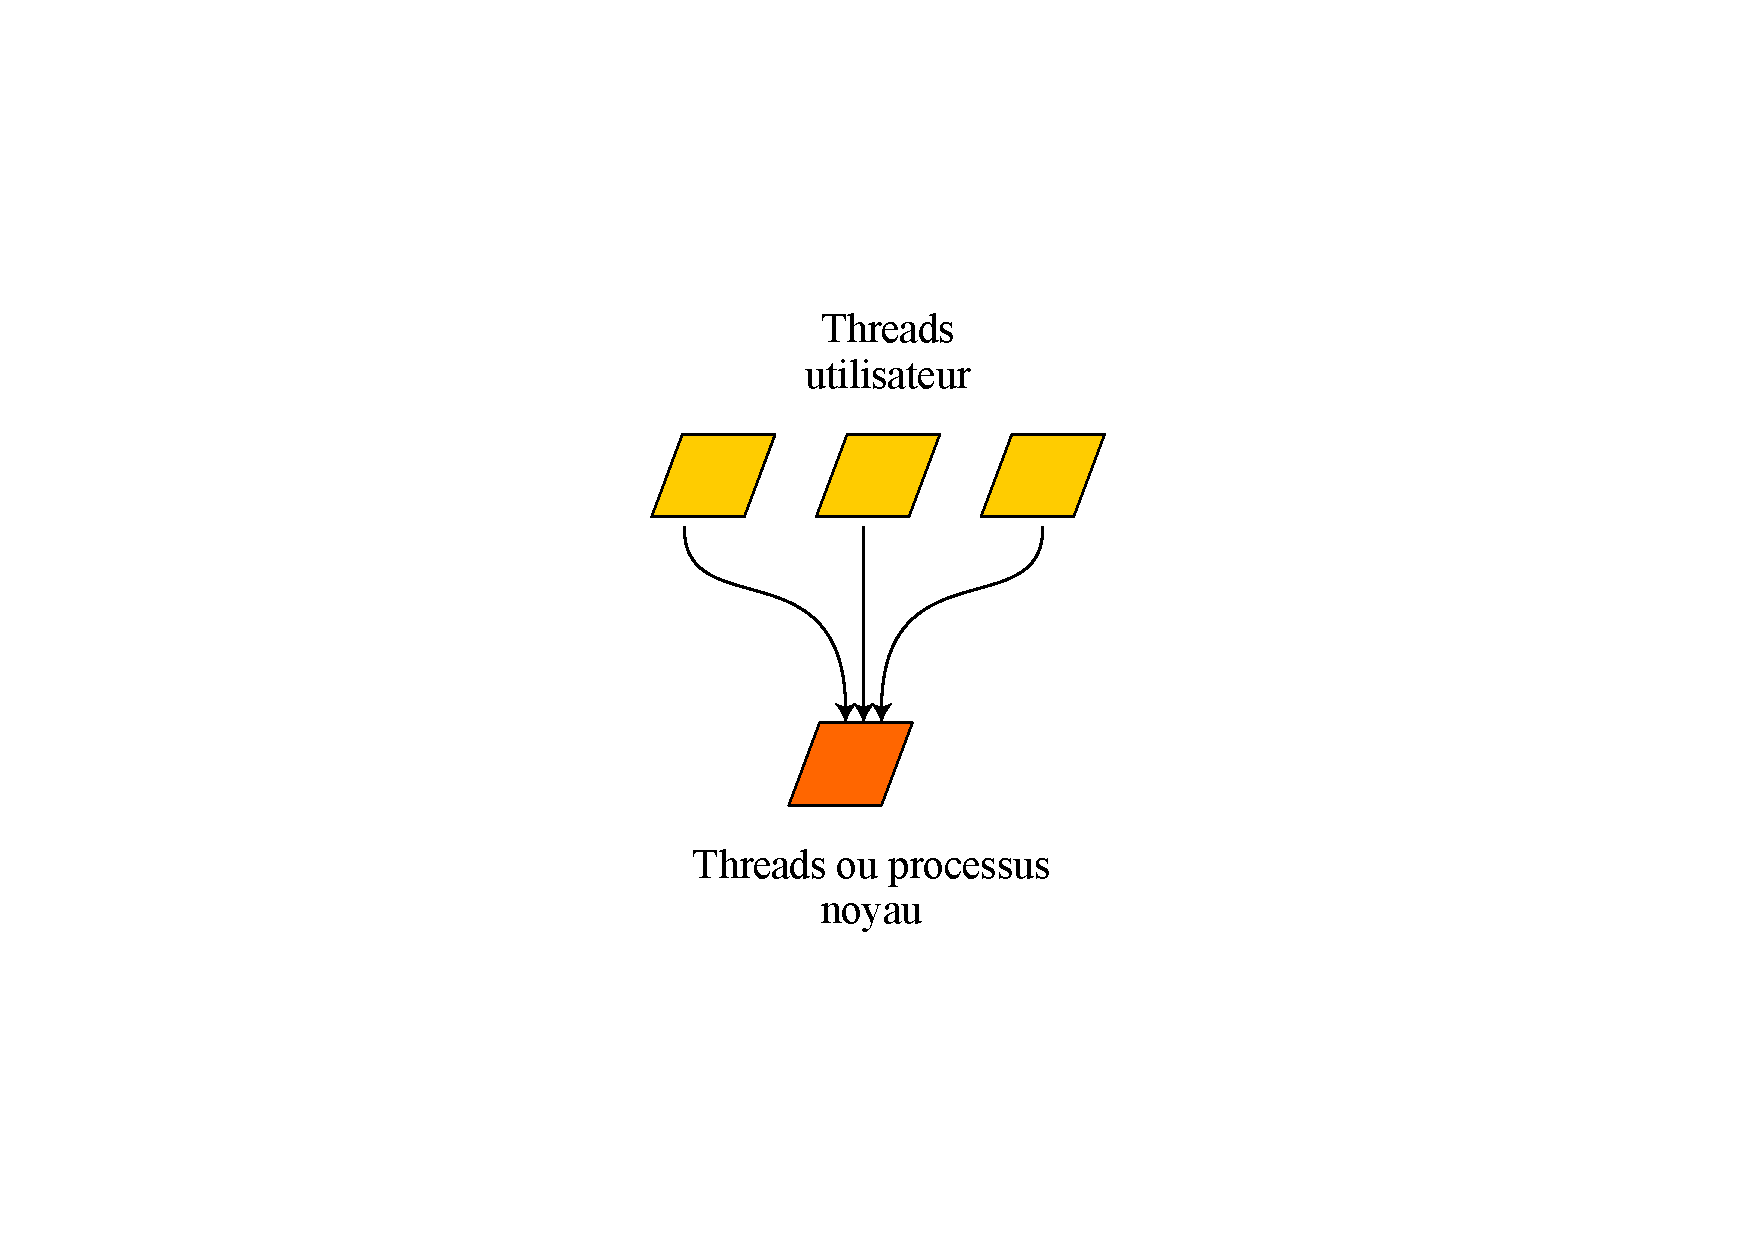
\includegraphics[width=4cm]{../illustration/threads-plusieurs-1.pdf}
 \end{columns}
\end{frame}


\begin{frame}
 \frametitle{Plusieurs vers un : un exemple}
 \begin{exampleblock}{Modèle \textit{green-thread} de Java}
 \begin{itemize}
 \item Thread non remontés au système
 \item La machine virtuelle gère tous les détails de l'API des threads
 \item Pour le système : 
 \begin{itemize}
 \item un processus / un flot d’exécution
 \item Le système ordonnance le processus de la JVM
 \item thread = abstraction interne à la machine virtuelle
 \end{itemize}
 \end{itemize}
 \end{exampleblock}
\end{frame}


\begin{frame}
 \frametitle{Le modèle ``un vers un''}
 \begin{columns}
 \column{0.5\textwidth}
 \begin{itemize}
 \item Threads indépendants identifiés par le système
 \begin{itemize}
 \item Plus de concurrence
 \item Possibilité de parallèlisation
 \item Surcoût de création et de gestion
 \end{itemize}
 \item Support :
 \begin{itemize}
 \item Solaris, Windows NT, Linux...
 \end{itemize}
 \end{itemize}
 \column{0.5\textwidth}
 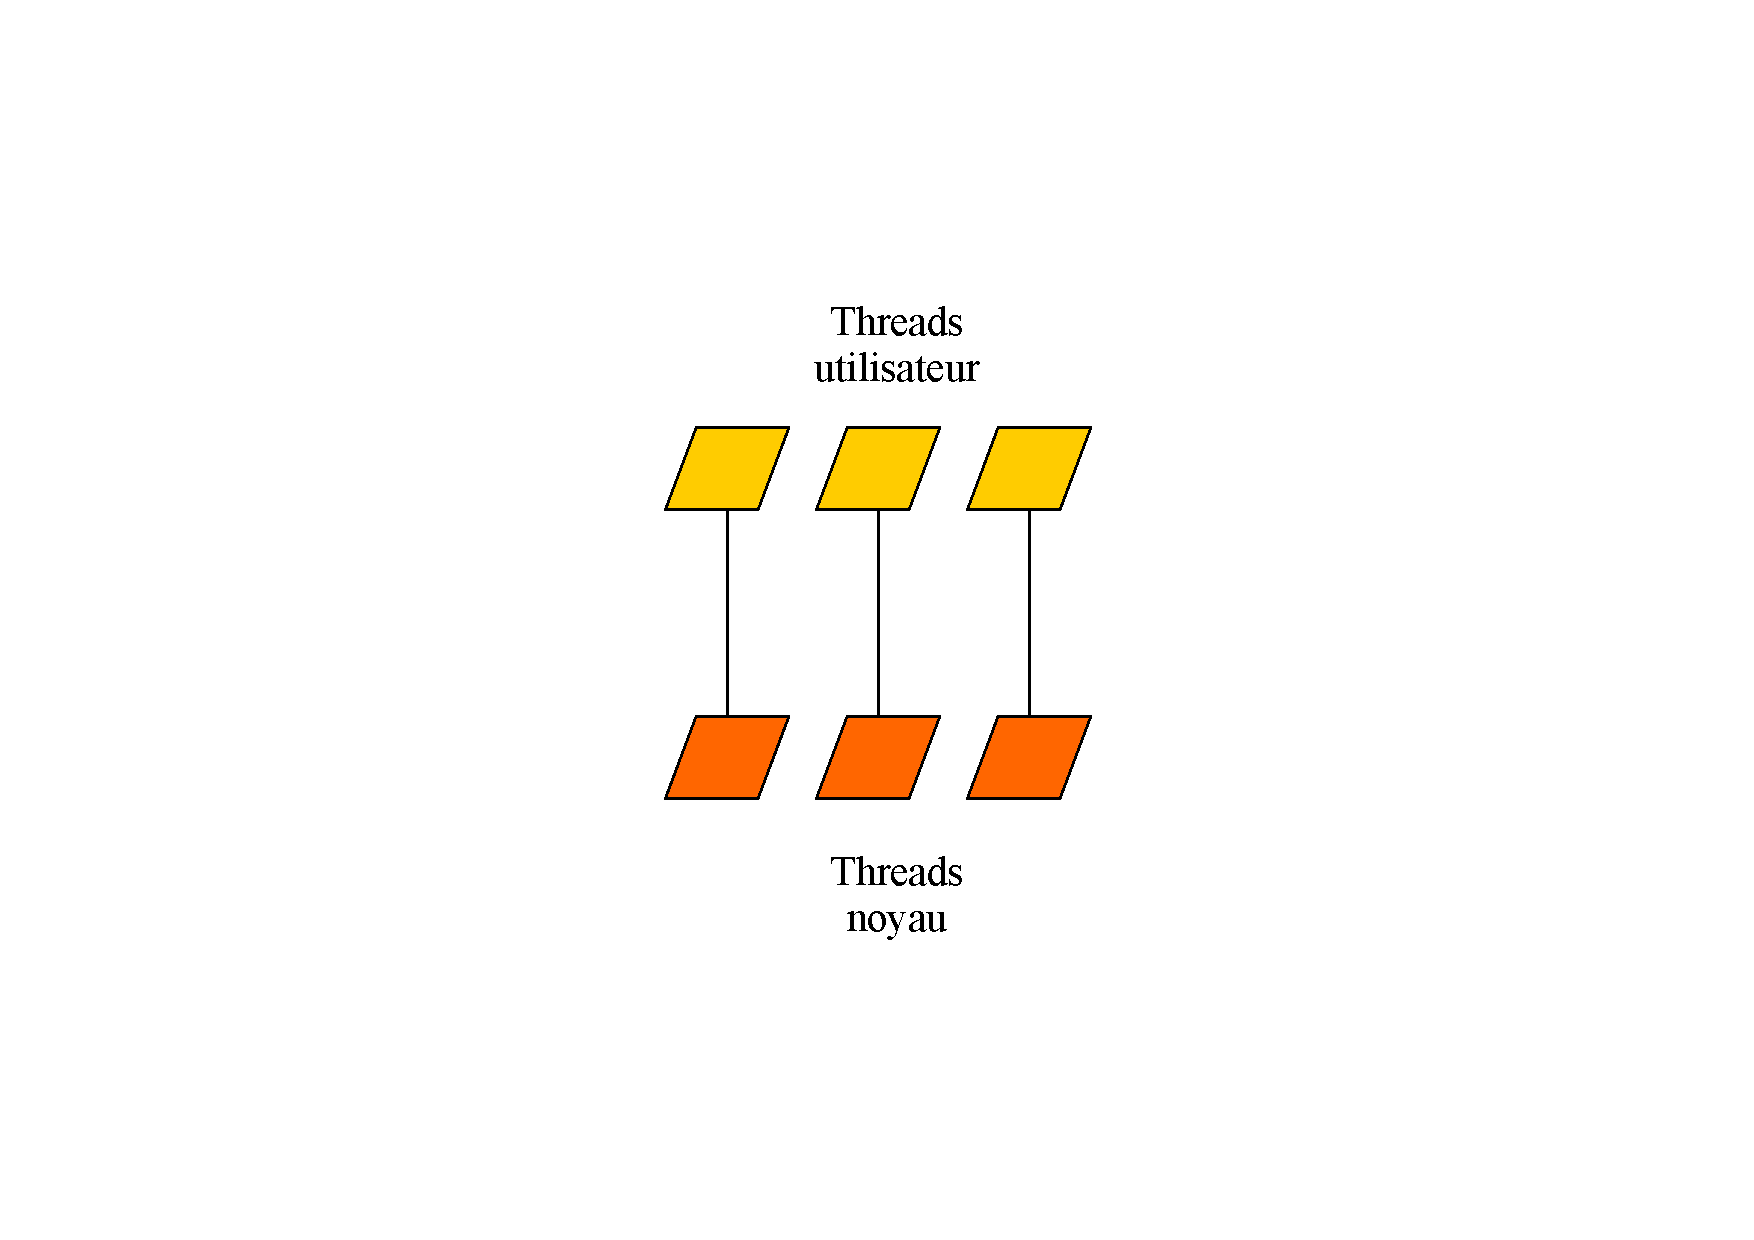
\includegraphics[width=4cm]{../illustration/threads-1-1.pdf}
 \end{columns}
\end{frame}


\begin{frame}
 \frametitle{Le modèle ``un vers un" : un exemple}
 \begin{itemize}
 \item Threads Java natifs sous Windows
 \item L’OS a entièrement connaissance des différents threads utilisés par la machine virtuelle
 \begin{itemize}
 \item 1 thread Java = 1 thread Windows
 \item Ordonnancement pris en charge par l’OS
 \end{itemize}
 \item Plus lourd que les green-threads
 \begin{itemize}
 \item Ordonnancement système vs JVM uniquement
 \end{itemize}
 \end{itemize}
\end{frame}


\begin{frame}
 \frametitle{Le modèle ``plusieurs vers plusieurs''}
 \begin{columns}
 \column{0.5\textwidth}
 \begin{itemize}
 \item Répartition de plusieurs threads utilisateurs sur un nombre inférieur ou égal de threads noyau
 \item Compromis
 \begin{itemize}
 \item Optimisation par le noyau
 \end{itemize}
 \item Support :
 \begin{itemize}
 \item Solaris, IRIX...
 \end{itemize}
 \end{itemize}
 \column{0.5\textwidth}
 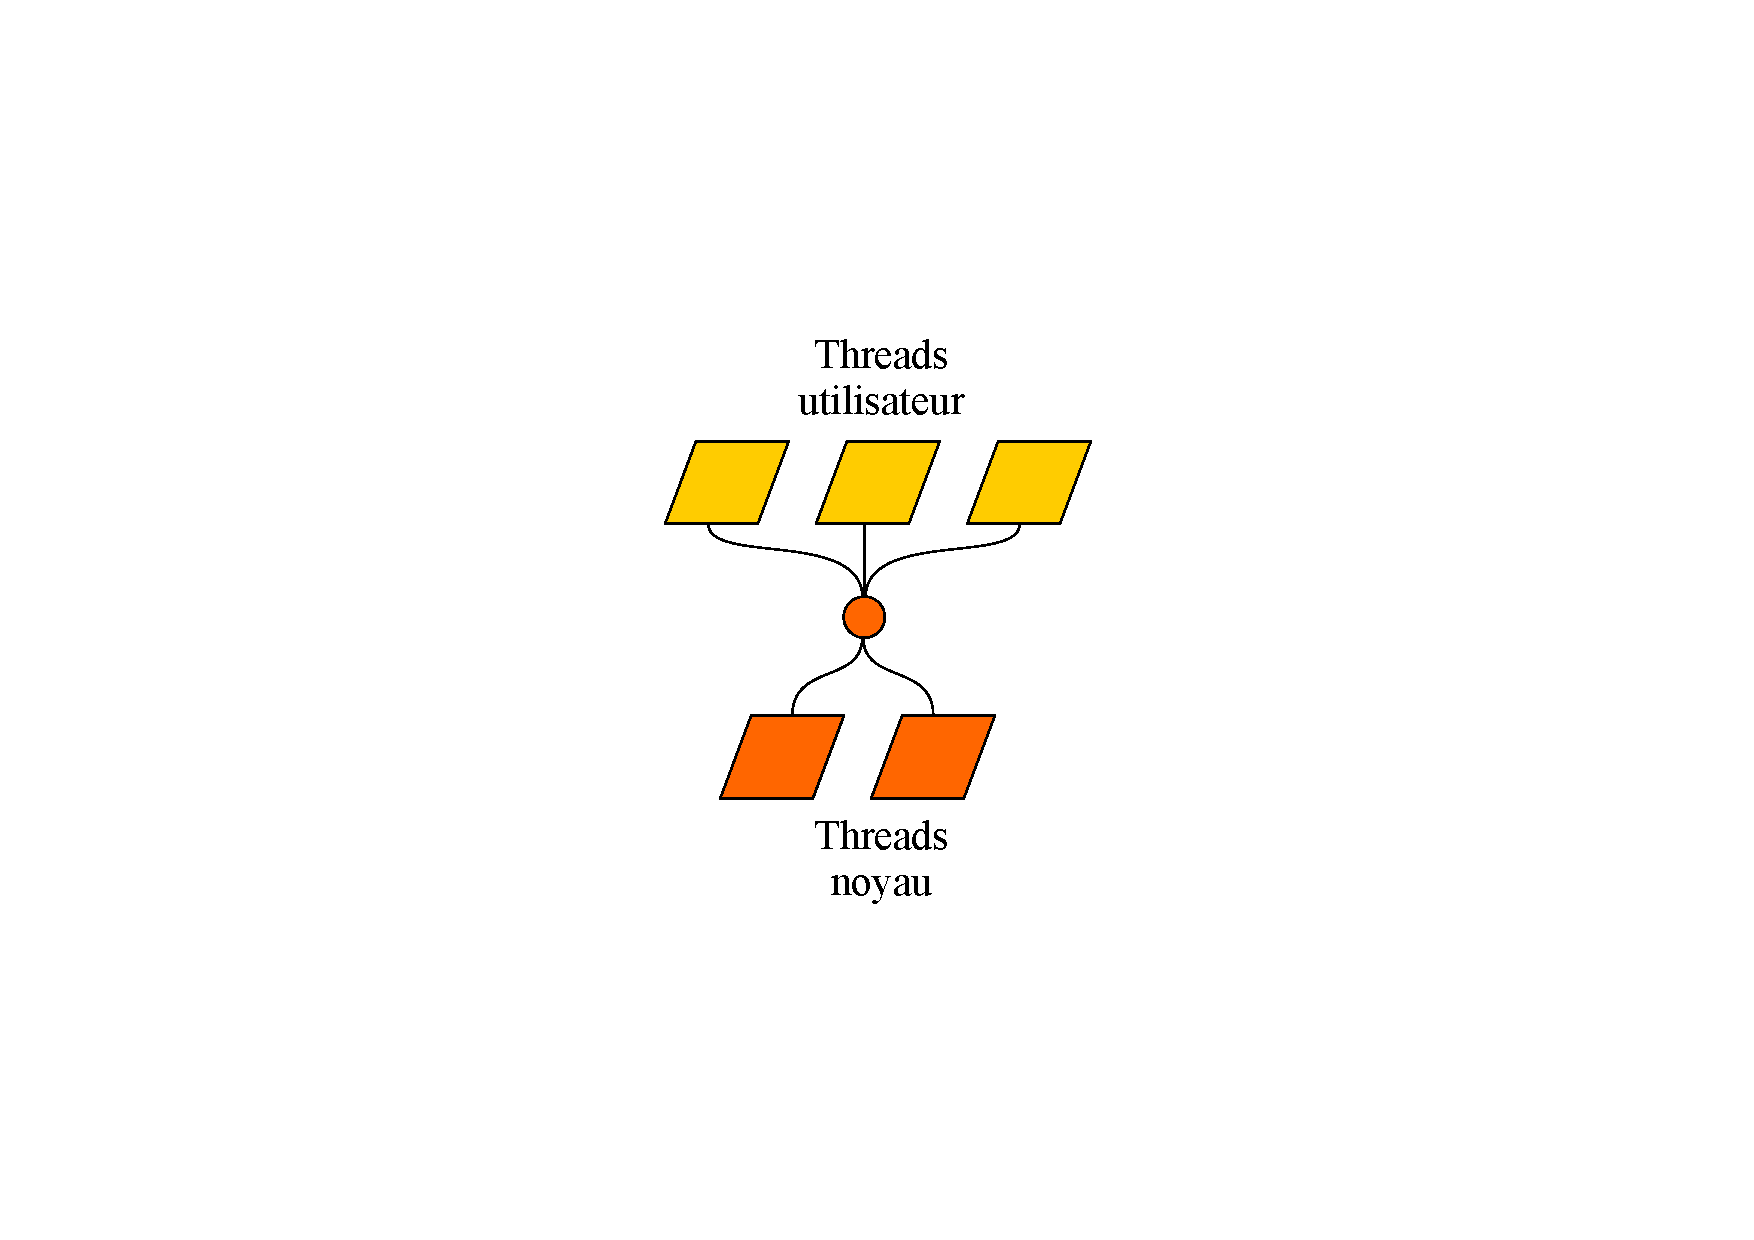
\includegraphics[width=4cm]{../illustration/threads-n-n.pdf}
 \end{columns}
\end{frame}


\begin{frame}
 \frametitle{Le modèle ``plusieurs vers plusieurs'' : un exemple}
 \begin{exampleblock}{Les LWP de Solaris (Lightweight Process)}
 \begin{itemize}
 \item Deux niveaux de threads :
 \begin{itemize}
 \item Les threads utilisateurs, inconnus du système
 \item Les threads du niveau système (LWP)
 \end{itemize}
 \item Affectation de LWP aux threads utilisateurs en fonction des besoins
 \begin{itemize}
 \item Liaison d’un thread utilisateur avec un LWP pendant le traitement d’appel système
 \item Création et affectation des LWP géré par l’OS
 \end{itemize}
 \end{itemize}
 \end{exampleblock}
\end{frame}


\frame[allowframebreaks]
{
\frametitle{Bibliographie}
\bibliographystyle{plain}
\bibliography{smb137}
}

\end{document}
